%% ch04_credit_risk.tex -- generated from credit_risk_interview_case_study_full.md
%% Do not edit by hand; edit the markdown and re-run build_tex.py.

\chapter{Credit Risk Assessment Agent}
\label{chap:ch04_credit_risk}

% \section*{Chapter Purpose}
% \addcontentsline{toc}{section}{Chapter Purpose}
% \label{sec:ch04_credit_risk-chapter-purpose}

% This chapter presents the credit risk assessment use case as a natural interview-style discussion between an interviewer and a candidate. The interviewer starts with a vague business problem and gradually reveals the true business context, requirements, constraints, and expectations. The candidate does not jump into architecture immediately. Instead, the candidate first clarifies the business need, then confirms functional and non-functional requirements, and only after that proposes the solution, reasoning, data design, system design, evaluation approach, and implementation details.

% The solution described here is aligned to a practical implementation in which a single FastAPI application orchestrates PDF ingestion, page indexing, tool-based extraction, deterministic financial calculations, scoring, memo generation, human review, and auditability.

% \medskip\hrule\medskip
\section{Business Context and Stakeholders}
\label{sec:ch04_credit_risk-1-business-context-and-stakeholders}

\speaker{Interviewer}{Let's solve a problem. A bank wants to speed up credit assessment for business borrowers. Today, analysts spend a lot of time reading financial statements and writing internal notes. Can you design a system for this?}

\speaker{Candidate}{Yes, definitely. Before proposing a solution, can you brief me a bit about the business context of credit risk here? For example, where exactly this process is used, who uses it, and what output the bank expects from the process?}

\speaker{Interviewer}{Fair question. This is used in the corporate and commercial lending journey. When a business customer applies for a new facility, renewal, enhancement, or restructuring, the relationship team collects financial statements and supporting documents. Credit analysts then review those documents, calculate ratios, understand risk, and write a credit memo for internal review.}

\speaker{Candidate}{That helps. So the credit memo is not customer-facing. It is an internal decision-support document used by the credit team and probably the committee as well, right?}

\speaker{Interviewer}{Correct. The credit memo is used internally by relationship managers, credit analysts, sanctioning authorities, and sometimes the credit committee.}

\speaker{Candidate}{Understood. One more important clarification: should the system only help analysts prepare the memo, or should it autonomously approve or reject the borrower?}

\speaker{Interviewer}{It should not autonomously approve or reject. It can draft the memo, assign a proposed rating, estimate risk, and recommend a decision, but a human must review and approve it.}

\speaker{Candidate}{Good. That means this is a decision-support agent, not an autonomous credit approval engine. That distinction is very important in banking.}

\speaker{Interviewer}{Exactly. The bank wants speed, consistency, and better traceability, but it does not want to remove human accountability.}

\speaker{Candidate}{Great. Then I would frame the business problem like this: the bank has a manual credit assessment workflow where analysts read long financial documents, extract financial data, calculate ratios, review qualitative risk factors, and prepare a credit memo. The goal is to reduce analyst effort and turnaround time while keeping the process explainable, auditable, and under human control.}

\speaker{Interviewer}{Yes, that is the right framing.}

\subsection{Stakeholders}

\speaker{Candidate}{Before going deeper, let me list the stakeholders so I can keep the design aligned:}

\begin{enumerate}[leftmargin=\speakwid]
\item Relationship manager, who brings the borrower case.
\item Credit analyst, who reviews the case and prepares analysis.
\item Credit officer or approver, who checks the memo and risk recommendation.
\item Credit committee, for larger or riskier facilities.
\item Risk and policy teams, who define thresholds and approval logic.
\item Operations and technology teams, who maintain the platform.
\item Audit and compliance teams, who need traceability.
\item The borrower indirectly, because document quality and timeliness depend on what they submit.
\end{enumerate}
\speaker{Interviewer}{Good. That covers the operating stakeholders well.}
\speaker{Candidate}{With stakeholders clear, can we lock down the business requirements and success metrics for the borrower assessment next?}

\medskip\hrule\medskip
\section{Requirements and Success Metrics}
\label{sec:ch04_credit_risk-2-requirements-and-success-metrics}

\speaker{Interviewer}{Good. Now can you design the system?}

\speaker{Candidate}{I can, but before describing the solution, I want to make sure I have the exact business requirements. Otherwise the design may solve the wrong problem.}

\speaker{Interviewer}{Go ahead.}

\subsection{Functional Requirements Discovery}

\speaker{Candidate}{First, what exactly goes into the system as input? Are we talking only about audited annual reports, or also interim financials, facility request letters, debt schedules, and covenant documents?}

\speaker{Interviewer}{Primarily PDF documents. Typical inputs are audited annual reports, interim financials if the latest audit is old, facility request letters, debt schedules, and covenant-related supporting documents.}

\speaker{Candidate}{Are the documents always PDF with searchable text, or can they be scanned images as well?}

\speaker{Interviewer}{Assume PDF only with text extractable from the pages. Scanned image-only PDFs are out of scope for now.}

\speaker{Candidate}{That is important. So the system should fail clearly if there is no text layer instead of pretending to understand the document.}

\speaker{Interviewer}{Correct.}

\speaker{Candidate}{What should the system produce at the end?}

\speaker{Interviewer}{It should produce a structured credit assessment result with extracted financial line items, ratios, benchmark comparison, trend analysis, a scorecard, a draft credit memo, and a proposed decision. It should also support follow-up Q\&A and a human review action.}

\speaker{Candidate}{Should it store only the final memo, or should it also persist intermediate outputs for audit and debugging?}

\speaker{Interviewer}{It should store both final and intermediate structured outputs where possible.}

\speaker{Candidate}{Good. Can users rerun the case after correcting an input or giving an instruction?}

\speaker{Interviewer}{Yes. Rerun is required, and each rerun should create a new version linked to the previous one.}

\speaker{Candidate}{Nice. Is web research or market/news sentiment part of the mandatory workflow?}

\speaker{Interviewer}{Optional. If enabled, the system can do public web and news enrichment using the company name. If not available or not desired, the run should still complete.}

\speaker{Candidate}{Understood. So external enrichment is fail-soft, not fail-hard. Functional scope is clear now. Could you please state the non-functional requirements first, before I fix the design constraints?}

\subsection{Non-Functional Requirements Discovery}

\speaker{Interviewer}{Let me state the non-functional requirements first. These describe how the system must run for credit assessment, not specific behaviors:}

\begin{itemize}[leftmargin=\speakwid]
\item Performance: assessment requests must be accepted in under 2 seconds; full analysis may run asynchronously over several minutes with pollable status.
\item Security: borrower financials and memos must be encrypted at rest and in transit; access must be authenticated and the system must not autonomously approve credit.
\item Scalability: the platform must support concurrent assessments without blocking request acceptance.
\item Reliability: the system must maintain 99.9\% availability; ratios, scores, and grades must be deterministic and reproducible, every material value must carry page and document lineage, and results must remain draft until human approval.
\item Usability: the interface must follow standard accessibility rules and let analysts trace any memo statement back to its source page, rerun versions, and review Q\&A history.
\end{itemize}

\speaker{Candidate}{Understood. Based on those NFRs, I would fix the following design constraints:}

\begin{itemize}[leftmargin=\speakwid]
\item Separate fast request acceptance from slow background execution.
\item Keep ratios, thresholds, and rating logic deterministic and explainable; the LLM must not compute critical financial values.
\item Persist intermediate and final structured outputs with page and document lineage for audit.
\item Treat web and news enrichment as fail-soft so a run still completes without it.
\item Keep the system as a single application process and optimize for clarity and reproducibility rather than a premature microservice split.
\end{itemize}
\speakcont{Is that consistent with the NFRs?}

\speaker{Interviewer}{Yes.}

\subsection{Success Metrics}

\speaker{Candidate}{Let me propose success metrics. Please confirm if these fit.}

\subsubsection{Business Metrics}

\begin{itemize}[leftmargin=\speakwid]
\item Reduction in analyst turnaround time per credit case.
\item Reduction in manual data extraction effort.
\item Increase in memo drafting consistency.
\item Faster review cycles for repeatable cases.
\item Better traceability during audit and review.
\end{itemize}
\subsubsection{Technical Metrics}

\begin{itemize}[leftmargin=\speakwid]
\item Financial line-item extraction accuracy.
\item Ratio calculation correctness.
\item Scorecard reproducibility.
\item Memo completeness and factual grounding.
\item Unsupported-claim rate in the memo.
\item Percentage of fields with page-level lineage.
\item Rerun traceability by version.
\item System completion rate for valid submissions.
\end{itemize}
\subsubsection{Human Review Metrics}

\begin{itemize}[leftmargin=\speakwid]
\item Reviewer override rate.
\item Approval versus rejection rate after review.
\item Correction frequency by field type.
\item Number of cases routed to validation review due to failures.
\end{itemize}
\speaker{Interviewer}{Yes. Add one more: the result should always remain a draft until a human reviewer approves or rejects it.}

\speaker{Candidate}{Absolutely. That becomes both a process rule and a metric around human control.}
\speaker{Candidate}{With requirements settled, shall we walk through the borrower data and document inputs the assessment will need?}

\medskip\hrule\medskip
\section{Data and Inputs}
\label{sec:ch04_credit_risk-3-data-and-inputs}

\speaker{Interviewer}{Good. Now walk me through what data you would need and how the system should treat it.}

\speaker{Candidate}{Sure. I would group the inputs into four layers.}

\subsection{Input Layer 1: User-Submitted Case Information}

\begin{itemize}[leftmargin=\speakwid]
\item Company name, optional but strongly recommended.
\item Ticker, optional and mainly useful for listed companies.
\item Search region for web enrichment.
\item A flag to enable or disable public web sentiment.
\item Requester identity for audit.
\item One or more PDF files.
\end{itemize}
\speaker{Interviewer}{What if the user submits no files?}

\speaker{Candidate}{Technically the pipeline can still create a case shell, but there will be nothing to extract. Ratios will remain null and the result will not be useful. So from a product perspective, files are effectively mandatory.}

\subsection{Input Layer 2: Document Pack}

\begin{itemize}[leftmargin=\speakwid]
\item Audited annual reports.
\item Interim or management accounts.
\item Facility request letter.
\item Debt schedule.
\item Covenant certificate.
\end{itemize}
\speaker{Interviewer}{Why do you care about debt schedule and covenant certificate separately if the annual report is already there?}

\speaker{Candidate}{Because the annual report may not reflect the current financing request or latest covenant status. Debt schedules and covenant certificates can provide maturity details, repayment pressure, and breach signals that strongly affect credit quality.}

\subsection{Input Layer 3: External Optional Enrichment}

\begin{itemize}[leftmargin=\speakwid]
\item Market and fundamentals from yfinance for listed entities.
\item Public web and news evidence using company name or aliases.
\item Sentiment and adverse information summarization based on collected evidence.
\end{itemize}
\speaker{Interviewer}{Would you let external data override the documents?}

\speaker{Candidate}{No. External data should only enrich or cross-check. It should never silently overwrite document-derived values. At most, it can fill missing values or raise discrepancy flags.}

\subsection{Input Layer 4: Internal Reference Data}

\begin{itemize}[leftmargin=\speakwid]
\item Ratio thresholds.
\item PD lookup table.
\item LGD by industry.
\item Grade bands.
\item Benchmark medians and quartiles by industry.
\end{itemize}
\speaker{Interviewer}{Why separate reference data from code?}

\speaker{Candidate}{Because policy thresholds and benchmark tables change more often than code architecture. Keeping them configurable allows business-controlled updates without rewriting the whole application.}
\speaker{Candidate}{With inputs and benchmarks clear, can I walk you through the end-to-end borrower assessment pipeline next?}

\medskip\hrule\medskip
\section{Solution Strategy and Pipeline Logic}
\label{sec:ch04_credit_risk-4-solution-strategy-and-pipeline-logic}

\speaker{Interviewer}{Good. Now can you explain the solution end to end?}

\speaker{Candidate}{Yes. I would design the system around one core principle:}

\begin{quote}
The LLM reads text and writes explanations. Python calculates everything that matters.
\end{quote}
\speakcont{This means the LLM is used where language understanding helps, but deterministic code owns ratios, scoring, grade mapping, PD, LGD, expected loss, and decision logic.}

\speaker{Interviewer}{Why are you making that separation so strongly?}

\speaker{Candidate}{Because in credit risk, the bank must be able to reproduce the same output for the same input pack, reference tables, and model version. If the LLM computes ratios or rating logic directly, the system becomes harder to trust, harder to audit, and harder to validate.}

\subsection{End-to-End Pipeline}

\speaker{Candidate}{The flow would look like this:}

\begin{enumerate}[leftmargin=\speakwid]
\item Accept the request quickly.
\item Save uploaded PDFs.
\item Create a new assessment version record.
\item Mark the case as queued.
\item Run the heavy work in the background.
\item Split PDFs into text-bearing pages.
\item Index those pages with embeddings in pgvector.
\item Run extraction agents over the indexed pages.
\item Optionally enrich with market and web data.
\item Compute ratios deterministically.
\item Compare ratios with benchmarks and analyze trends.
\item Score the case using a deterministic scorecard.
\item Draft the memo using the compact, computed assessment.
\item Persist results atomically.
\item Mark the result as awaiting review.
\item Support review, Q\&A, and rerun.
\end{enumerate}
\subsection{End-to-End Flow Diagram}

\begin{figure}[htbp]
\centering
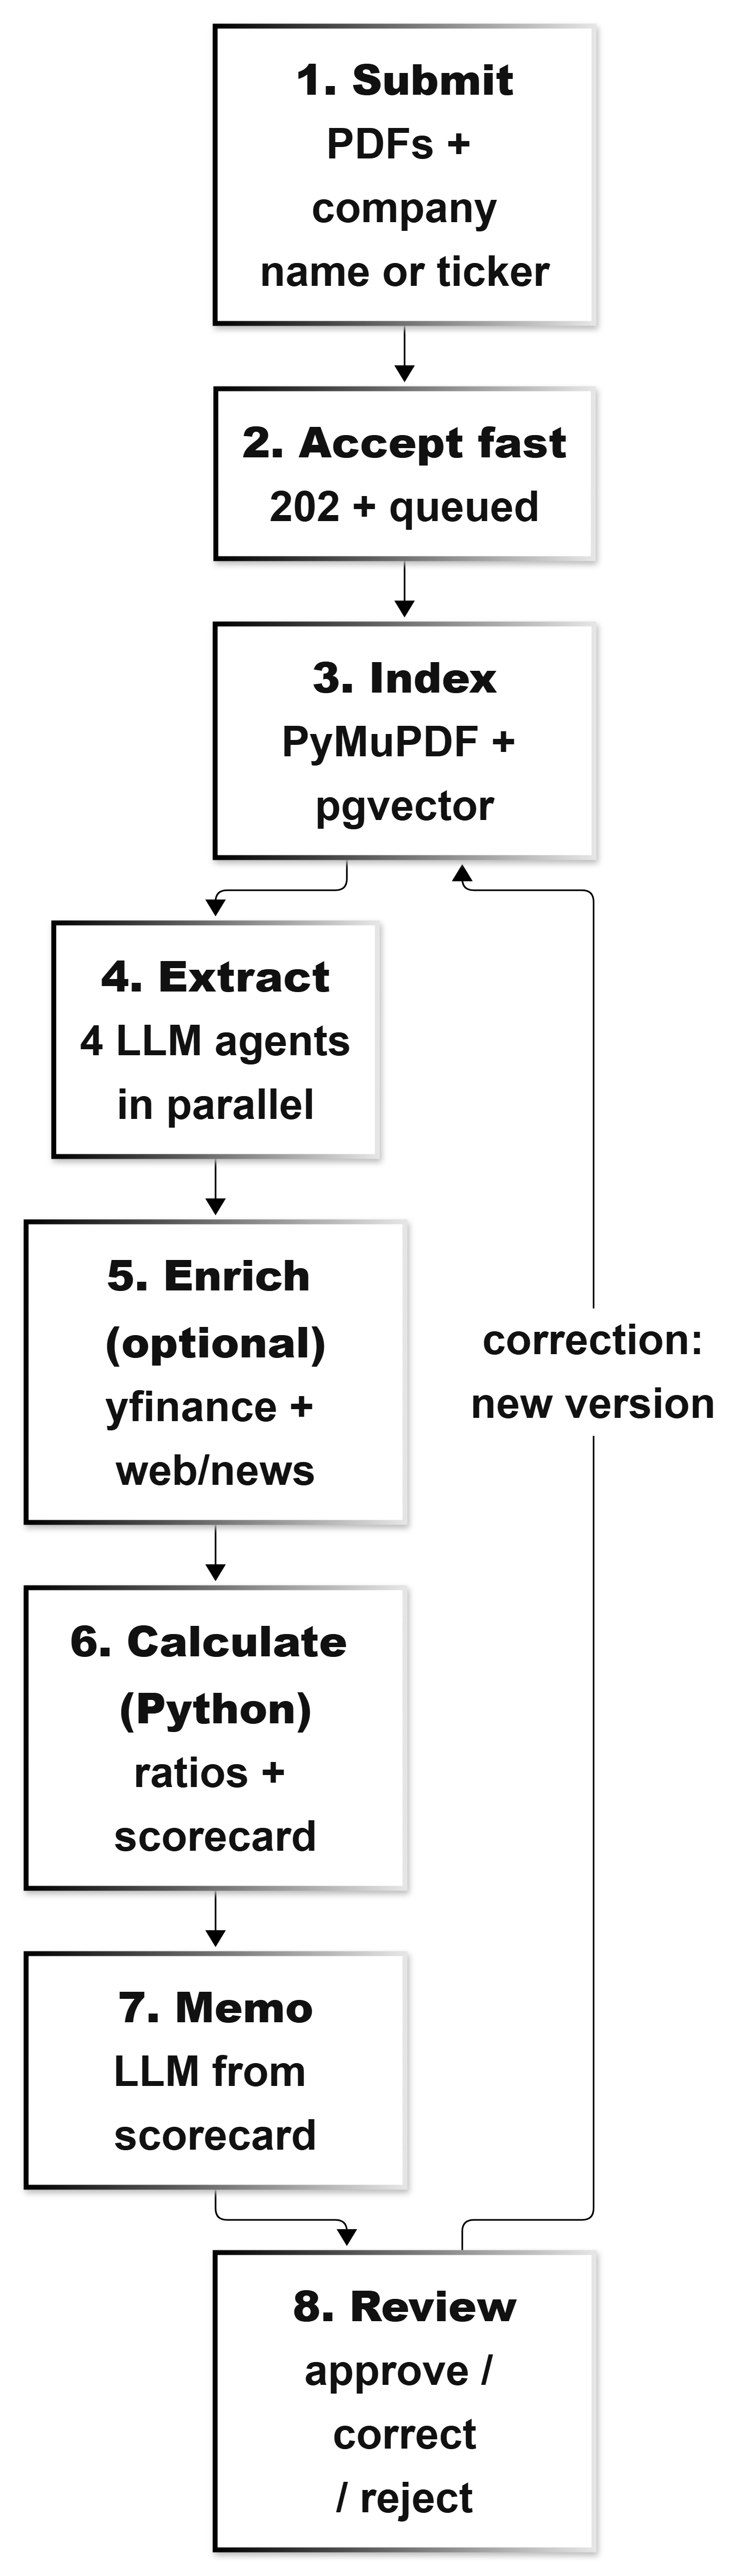
\includegraphics[width=\textwidth,height=0.85\textheight,keepaspectratio]{../diagrams/credit_risk/01_flowchart_end-to-end-flow-diagram.png}
\caption{End-to-End Flow Diagram}
\label{fig:ch04_credit_risk-01-flowchart-end-to-end-flow-diagram}
\end{figure}

\speaker{Interviewer}{Why do you index pages instead of giving the whole PDF directly to the LLM?}

\speaker{Candidate}{Three reasons. First, large packs may be long and expensive to send whole. Second, tool-based retrieval forces the model to search relevant pages instead of hallucinating over too much context. Third, page-level indexing supports lineage and selective retrieval.}

\subsection{Main Agents and Components}

\speaker{Candidate}{I would structure the logic using a few focused agents and deterministic services.}

\subsubsection{Tool-Based Extractors}

\begin{enumerate}[leftmargin=\speakwid]
\item Company metadata extractor.
\item Financial line-item extractor.
\item Notes and contingencies extractor.
\item Facility request extractor.
\end{enumerate}
Each one gets only two tools:

\begin{itemize}[leftmargin=\speakwid]
\item \texttt{search\_pages(query, k)}
\item \texttt{get\_page(page\_number)}
\end{itemize}
So instead of passing raw PDFs, we let the extractor search the indexed document pack and then return strict JSON.

\speaker{Interviewer}{Why four separate extractors instead of one big extractor?}

\speaker{Candidate}{Because each task has different search behavior, different schema, and different failure modes. A single extractor tends to become too broad, less reliable, and harder to debug. Separate extractors also allow parallel execution.}

\subsubsection{Deterministic Services}

\begin{itemize}[leftmargin=\speakwid]
\item Unit normalization.
\item Period grouping.
\item Derived values such as EBITDA or total debt where safely defined.
\item Ratio calculations.
\item Benchmark comparisons.
\item Trend analysis.
\item Scorecard computation.
\end{itemize}
\subsubsection{Optional Enrichment Services}

\begin{itemize}[leftmargin=\speakwid]
\item yfinance backfill for listed borrowers.
\item Web/news collection.
\item LLM-based public sentiment synthesis.
\end{itemize}
\subsubsection{Narrative Services}

\begin{itemize}[leftmargin=\speakwid]
\item Credit memo synthesis from compact scorecard JSON.
\item Follow-up Q\&A from the completed assessment JSON.
\end{itemize}
\subsubsection{Human Control}

\begin{itemize}[leftmargin=\speakwid]
\item Review action: approved, corrected, or rejected.
\item Rerun with instruction.
\item Full audit trace.
\end{itemize}
\speaker{Candidate}{With the pipeline overview set, shall we dig into the key design decisions behind each borrower assessment step?}

\medskip\hrule\medskip
\section{Deep Discussion on Pipeline Decisions}
\label{sec:ch04_credit_risk-5-deep-discussion-on-pipeline-decisions}

\subsection{Fast Accept and Background Execution}

\speaker{Interviewer}{Why not keep the HTTP connection open and return the final result when processing finishes?}

\speaker{Candidate}{Because credit assessment can take minutes when multiple extractor calls, indexing, and memo generation are involved. Browsers, proxies, and load balancers often terminate long idle connections. If that happens, the user may lose the assessment reference. So I would accept quickly, return the version ID, and let the client poll status.}

\speaker{Interviewer}{How would the status work?}

\speaker{Candidate}{I would maintain lightweight live phase tracking in Redis for states like queued, indexing documents, extracting financials, enriching and scoring, writing memo, done, and failed. Postgres remains the source of truth; Redis just improves responsiveness for status polling.}

\subsection{Background Processing Sequence}

\begin{figure}[htbp]
\centering
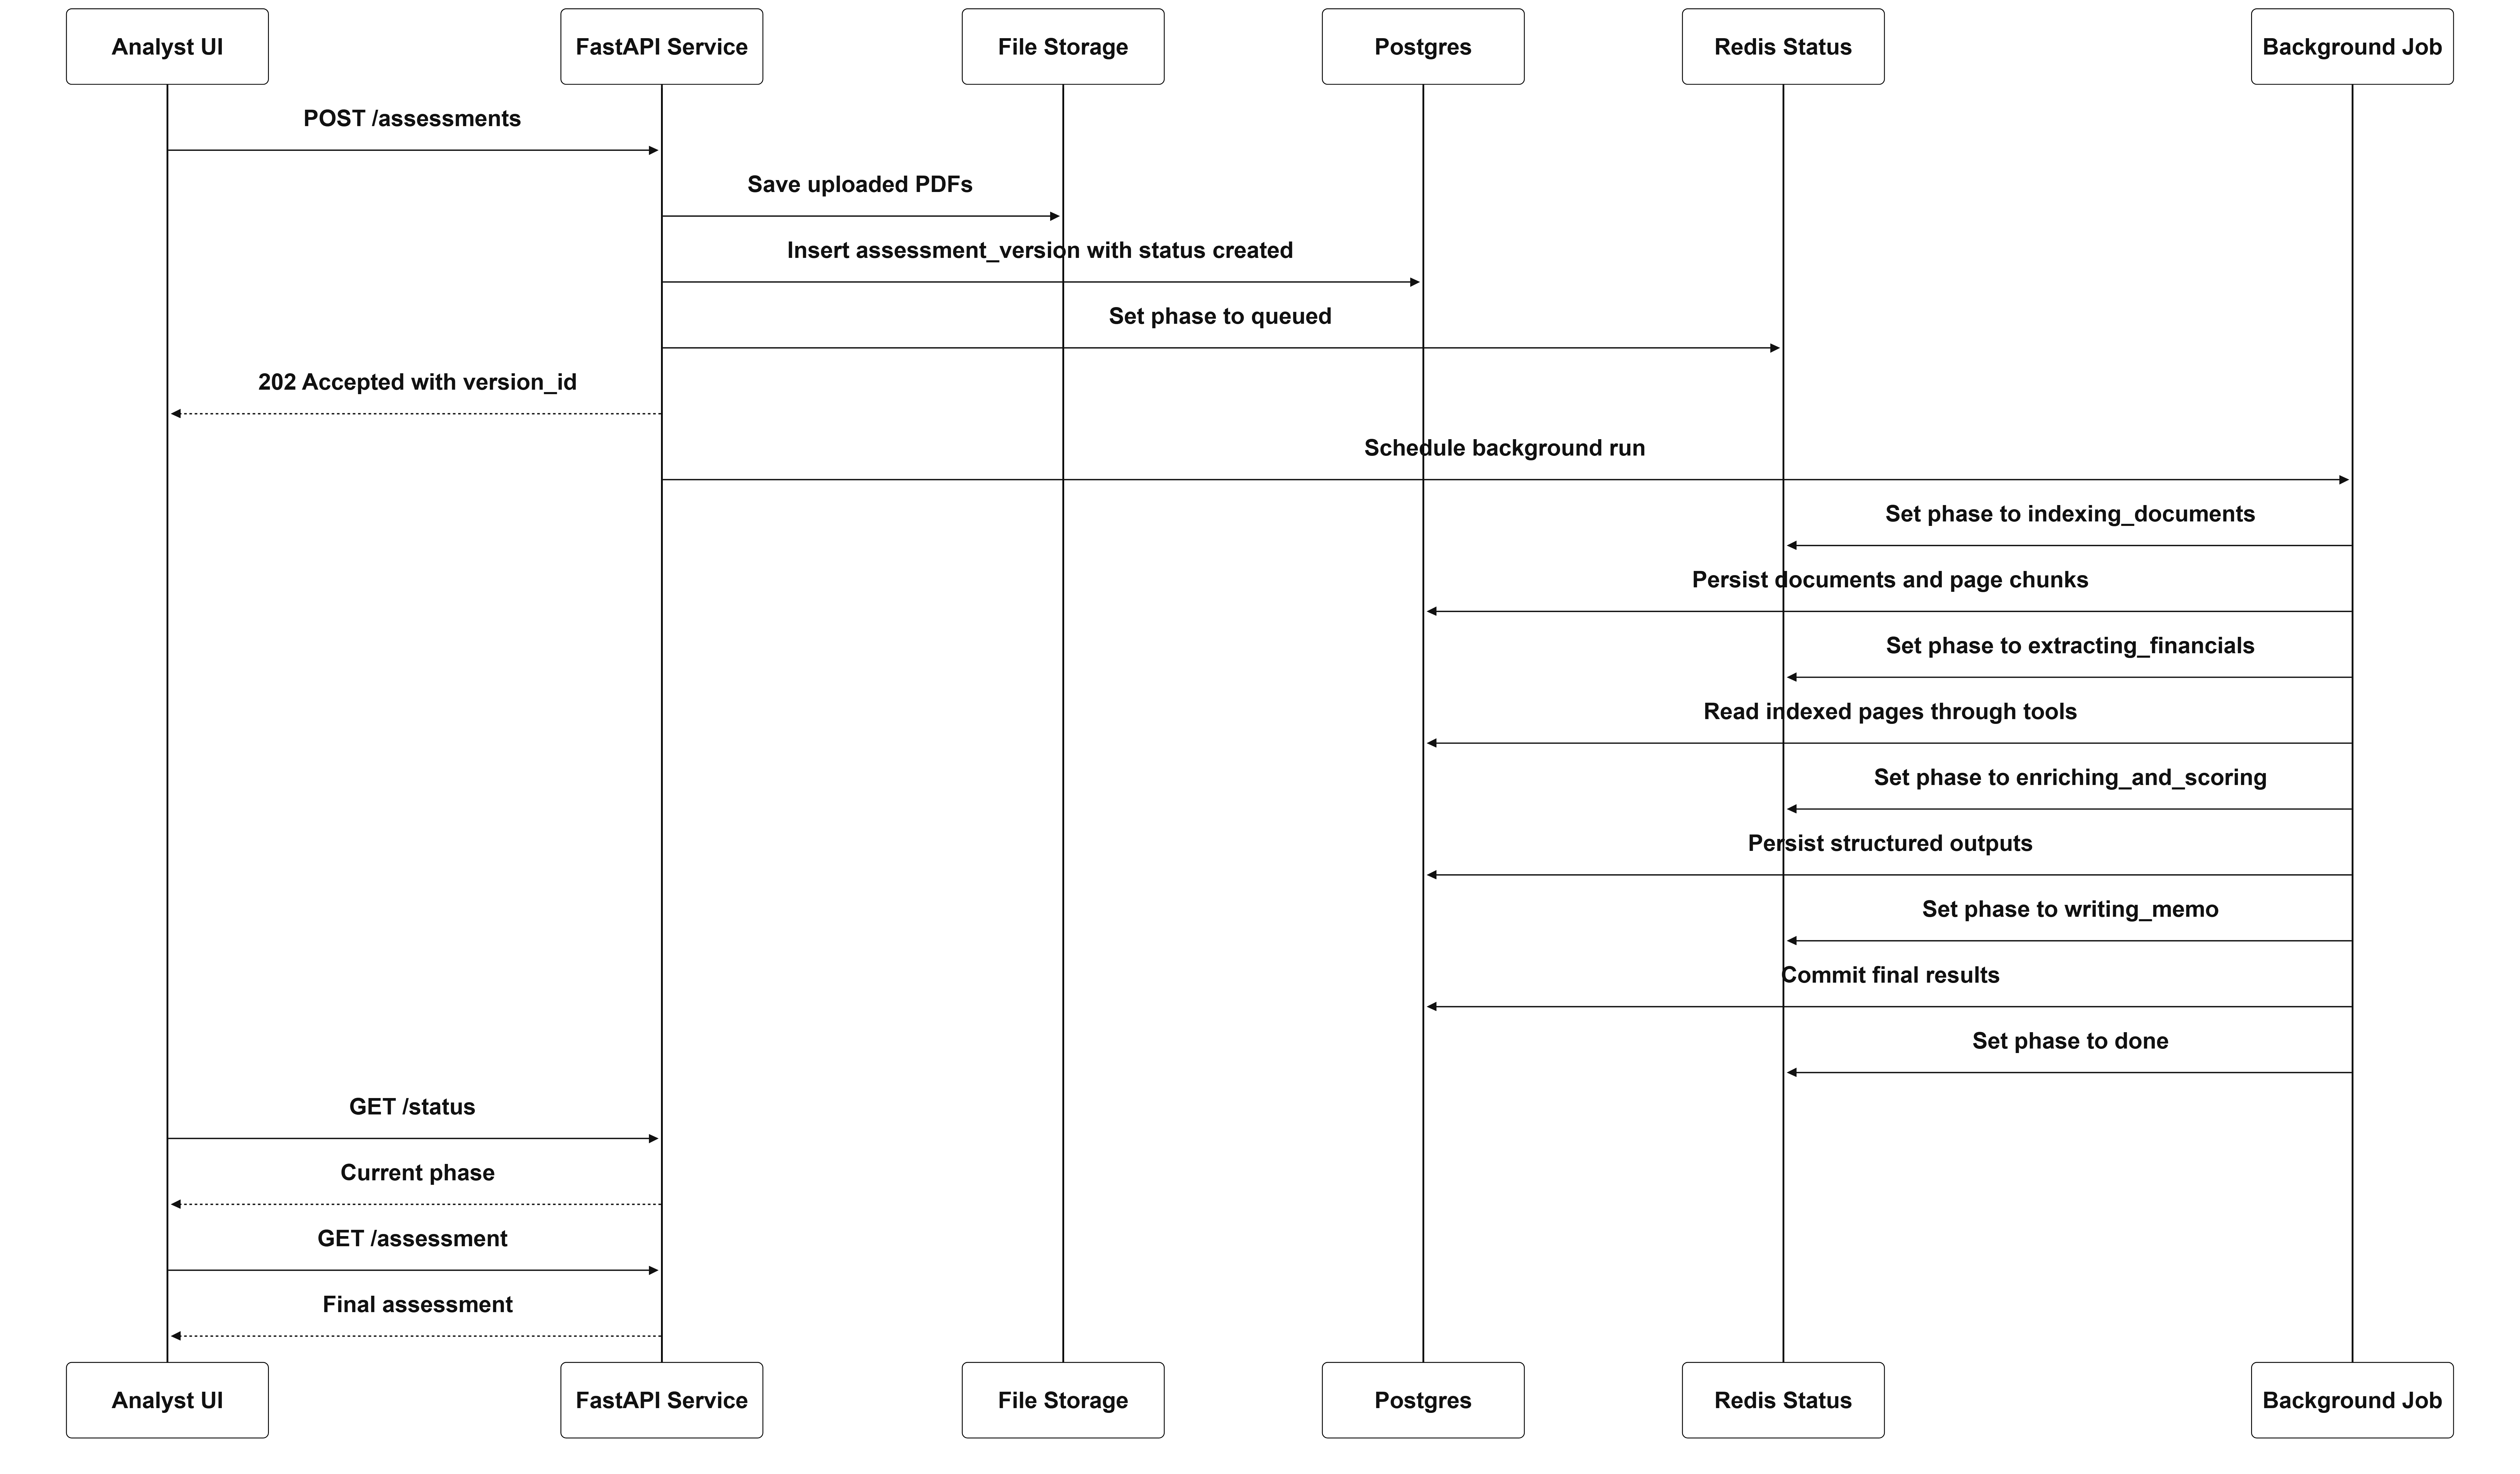
\includegraphics[width=\textwidth,height=0.85\textheight,keepaspectratio]{../diagrams/credit_risk/02_sequenceDiagram_background-processing-sequence.png}
\caption{Background Processing Sequence}
\label{fig:ch04_credit_risk-02-sequencediagram-background-processing-sequence}
\end{figure}

\subsection{PDF Processing}

\speaker{Interviewer}{Why do you reject image-only scanned PDFs?}

\speaker{Candidate}{Because my design uses PyMuPDF text extraction and assumes a text layer. If there is no extractable text, forcing the rest of the pipeline to continue would create silent garbage. A clean failure is better than false confidence.}

\speaker{Interviewer}{How are pages numbered when there are multiple PDFs?}

\speaker{Candidate}{I would use global numbering across the uploaded pack. For example, document one may occupy pages 1--35 and document two continues from 36 onward. That simplifies tool access and page referencing across the combined pack.}

\subsection{Why Tool Calling?}

\speaker{Interviewer}{Why use tool calling at all? Why not just retrieve the top few pages yourself and pass them to the model?}

\speaker{Candidate}{Tool calling gives the extractor autonomy to search iteratively. For example, the company metadata agent may first search for the principal activities page, then separately search the auditor's report page, then maybe open one specific page in full. This makes extraction more robust than a fixed retrieval heuristic. But I would still bound the loop, for example with a six-turn maximum, so it remains predictable.}

\speaker{Interviewer}{What if the model keeps calling tools forever or chooses irrelevant queries?}

\speaker{Candidate}{I would cap the maximum iterations. After the limit, I would instruct it to stop searching and answer with the best structured JSON it can produce from the retrieved content. That creates bounded cost and avoids infinite loops.}

\subsection{Tool-Calling Extraction Sequence}

\begin{figure}[htbp]
\centering
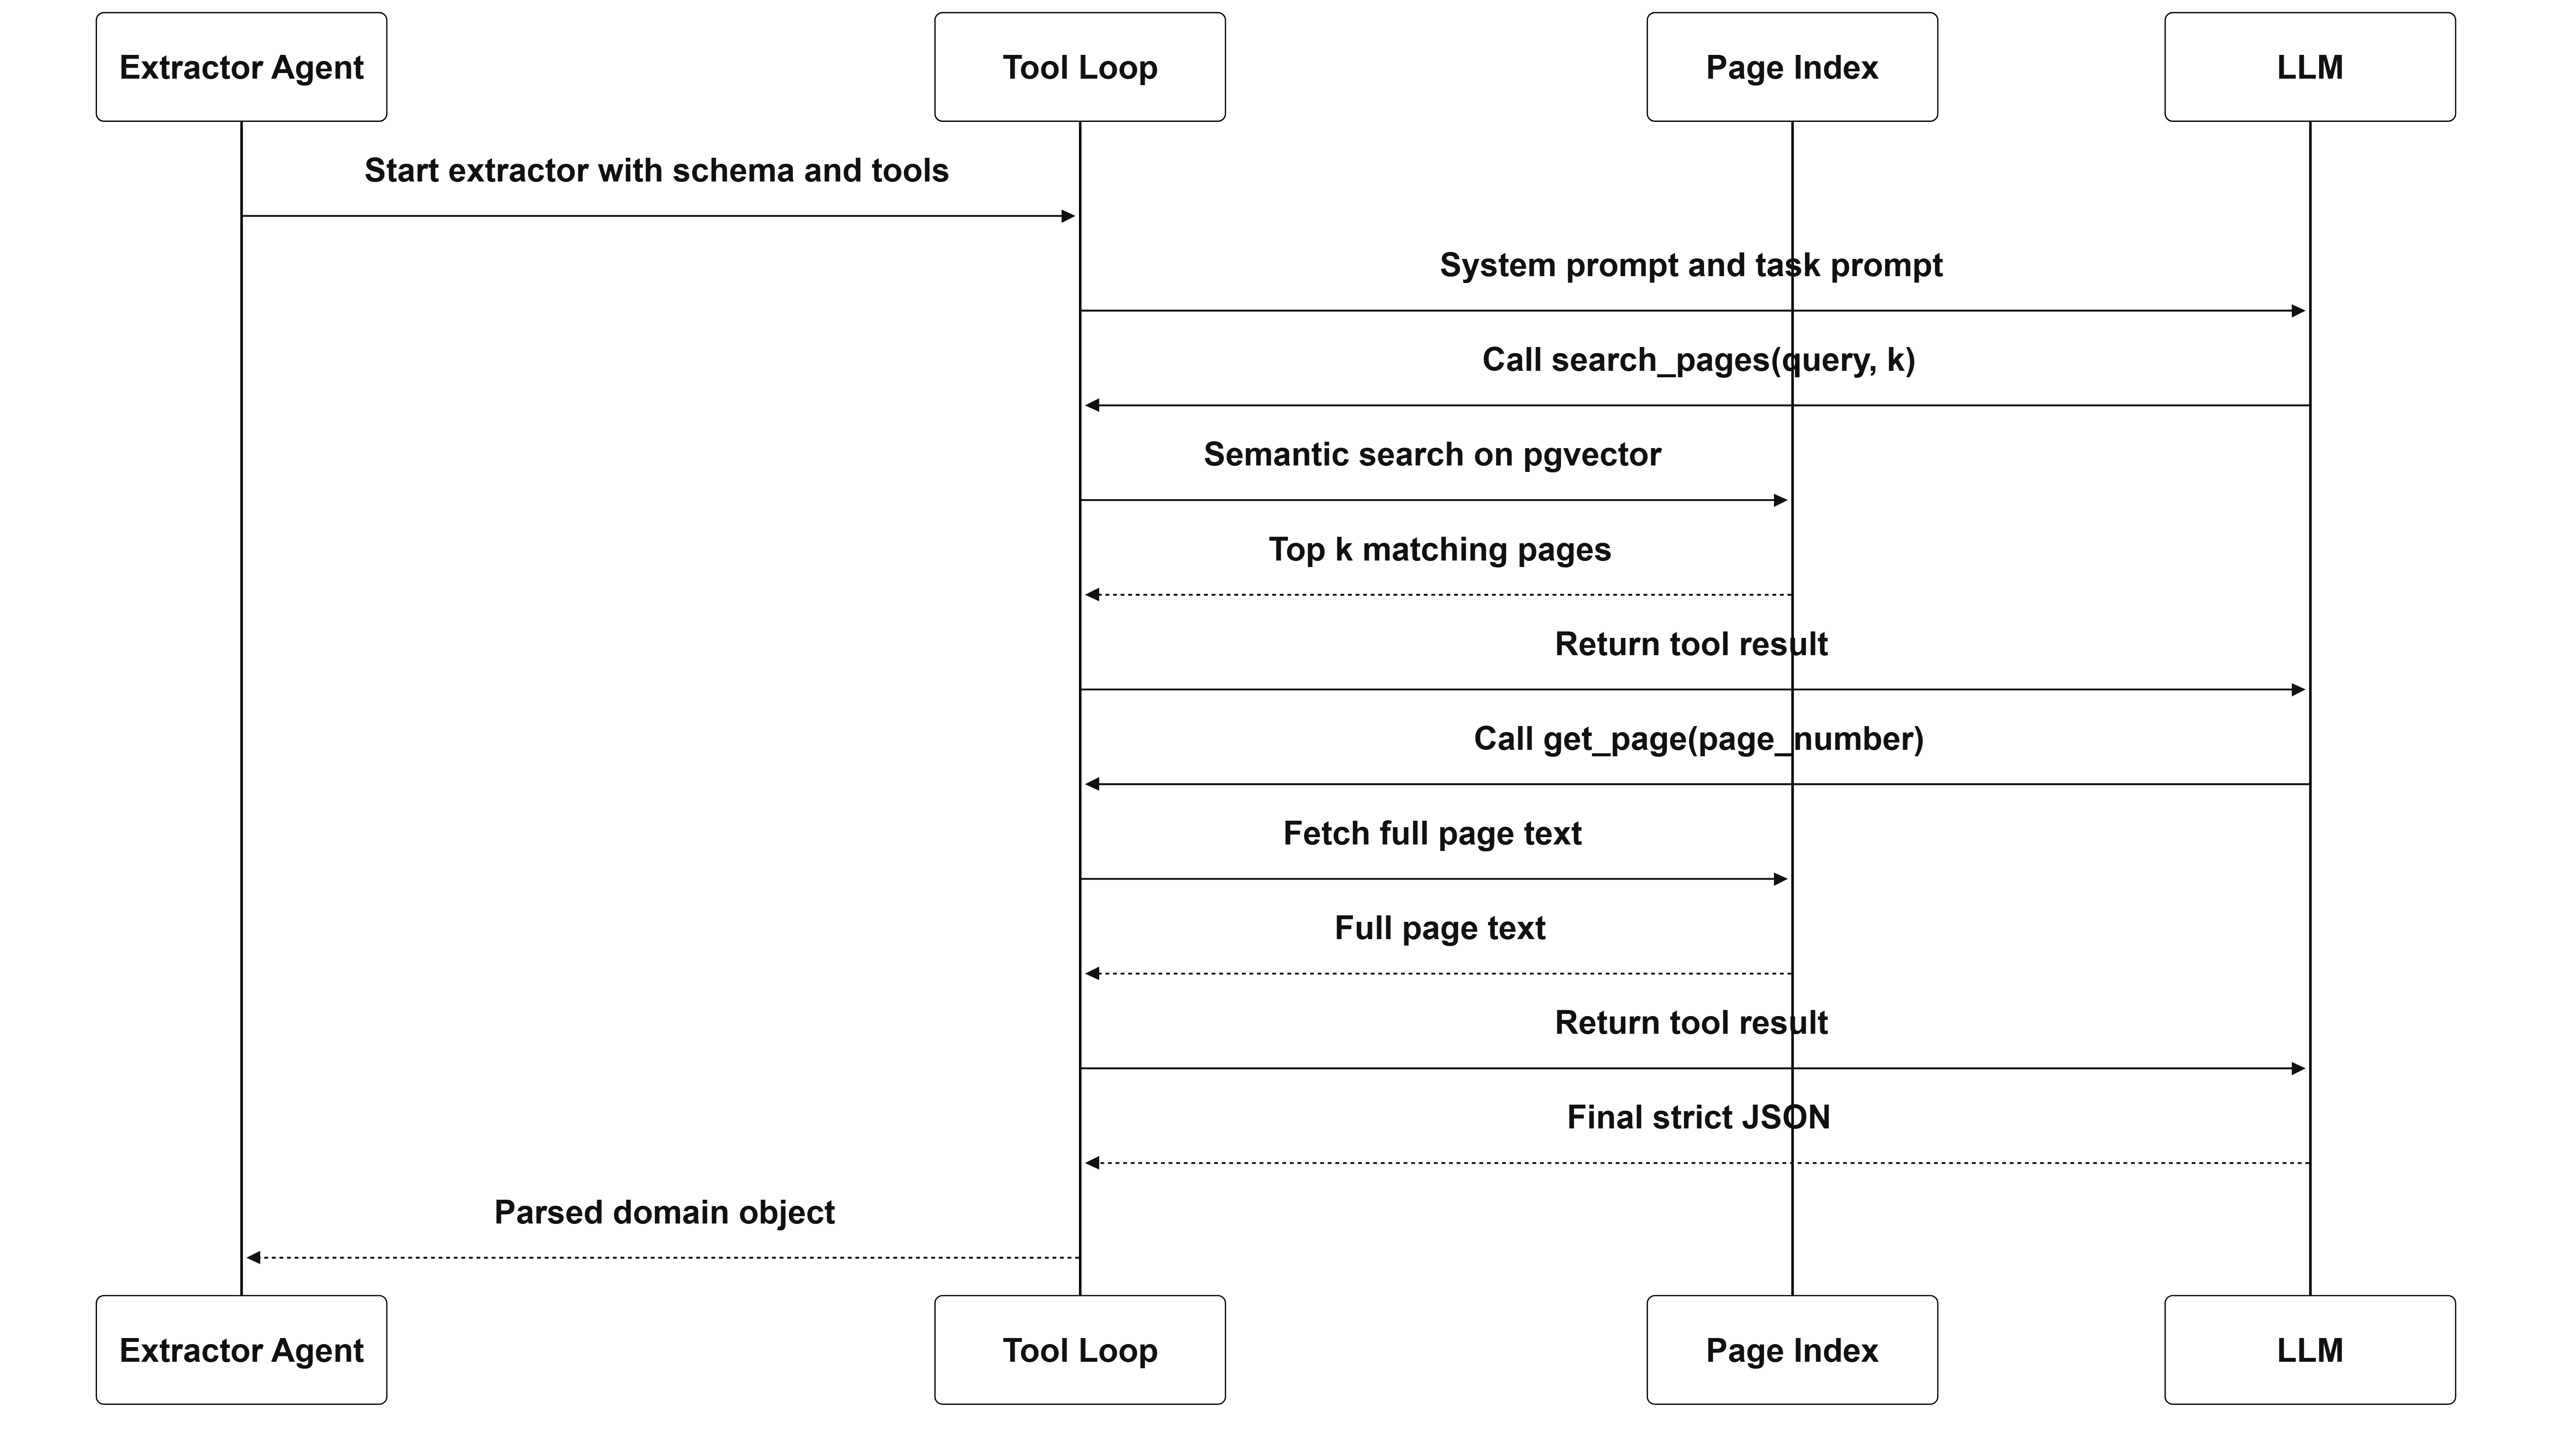
\includegraphics[width=\textwidth,height=0.85\textheight,keepaspectratio]{../diagrams/credit_risk/03_sequenceDiagram_tool-calling-extraction-sequence.png}
\caption{Tool-Calling Extraction Sequence}
\label{fig:ch04_credit_risk-03-sequencediagram-tool-calling-extraction-sequence}
\end{figure}

\subsection{Financial Line-Item Extraction}

\speaker{Interviewer}{This feels like the most important part. How would the line-item extractor work in depth?}

\speaker{Candidate}{I would make it extract one record per line item per period. That means revenue for FY2023 and revenue for FY2022 become separate records. I would also standardize labels to a controlled vocabulary such as revenue, EBIT, EBITDA, total debt, total equity, operating cash flow, and so on.}

\speaker{Interviewer}{Why insist on one record per item per period?}

\speaker{Candidate}{Because ratio calculations are period-specific. If the extractor mixes multiple periods into one object, downstream deterministic logic becomes messy and error-prone.}

\speaker{Interviewer}{Would the LLM be allowed to sum or derive missing values during extraction?}

\speaker{Candidate}{No. During extraction, the model should transcribe only what is printed. It should not invent, sum, or scale values. Scaling and derivation belong to deterministic post-processing. For example, if a statement is in thousands, the extractor captures the unit as thousands and Python normalizes later.}

\subsection{Correctness Gates for LLM Extraction}

\speaker{Candidate}{Before we leave extraction, can I go one level deeper on how we validate what the extractors return, beyond just checking the JSON shape?}

\speaker{Interviewer}{Yes, please. Schema checks alone would not tell us whether the values are actually right.}

\speaker{Candidate}{Exactly. Schema validation guarantees shape, not correctness. So behind the company-metadata and line-item extractors we add a small pure-Python correctness gate in \texttt{llm\_validation.py}. There are three scoring helpers. The classification check reports an estimated percent correct per row: whether the label is inside the allowed vocabulary, whether the source label is non-empty, and whether it overlaps with the retrieved page evidence. An unknown label costs roughly a 0.4-over-n penalty. The extraction check scores required-field presence, finite numerics below 1e15, and grounding of each label in evidence, and an empty output scores 0.0. The suggestion check requires non-empty actionable text of at least three words, with valid universe references and risk acknowledgement where required.}

\speaker{Interviewer}{And what happens when confidence is low?}

\speaker{Candidate}{Anything below a 0.50 confidence threshold lists the failed validations, appends them to the prompt through \texttt{build\_retry\_addendum()}, and reinvokes the model with a bounded retry of at most three attempts, keeping the best attempt fail-soft. For the credit workflow this matters because a misclassified audit opinion or a wrong period label would poison every downstream ratio, the scorecard severity, and the memo grounding. The retry tells the model precisely which rule it broke, for example a bad label or a missing period, so the second attempt fixes evidence grounding instead of repeating the mistake. The gate is wired into metadata extraction for the audit-opinion classification and into line-item extraction for label, period, and value completeness via \texttt{\_extract\_json\_validated()}, and it is covered by four offline tests that need no network.}

\subsection{Notes and Contingencies}

\speaker{Interviewer}{Why do notes matter so much? Many systems focus only on financial statements.}

\speaker{Candidate}{Because some high-risk signals live in notes rather than core statements. Going-concern language, guarantees, litigation, and contingent liabilities can materially change the decision even if ratios look decent. In this design, going-concern or certain adverse audit situations can trigger a hard stop.}

\subsection{Facility Request Extraction}

\speaker{Interviewer}{Why extract facility request details through the same document tools?}

\speaker{Candidate}{Because request amount, purpose, tenor, and facility type often appear in supporting documents rather than financial statements. Those fields influence the memo narrative and credit recommendation. If missing, I would allow nulls rather than guessing.}

\subsection{yfinance Backfill}

\speaker{Interviewer}{Tell me more about the yfinance enrichment. Why use it at all?}

\speaker{Candidate}{It can be useful for listed companies when document coverage is incomplete. For example, if the line-item extractor missed a period or a specific financial line, yfinance can fill missing values. But it should only fill blank cells, never overwrite document-derived numbers.}

\speaker{Interviewer}{What if yfinance disagrees with the annual report by 4 percent?}

\speaker{Candidate}{I would log a discrepancy if the delta exceeds a configured tolerance, such as 2 percent. The discrepancy becomes reasoning or audit information, not an automatic override.}

\subsection{Web and News Enrichment}

\speaker{Interviewer}{I am skeptical about web sentiment in credit risk. Why include it?}

\speaker{Candidate}{That skepticism is healthy. I would not let public web sentiment drive the decision on its own. It is only supporting color. If public evidence suggests litigation, regulatory trouble, layoffs, insolvency, or governance concerns, it can contribute as an adverse-media factor. But it must be clearly marked as optional, lower-confidence, and dependent on entity disambiguation.}

\speaker{Interviewer}{How do you avoid matching the wrong company with the same name?}

\speaker{Candidate}{I would explicitly ask the sentiment step to assess disambiguation confidence as low, medium, or high. If confidence is low, adverse findings should be discounted or capped. The system should never present weakly matched web evidence as confirmed borrower fact.}

\subsection{Optional Enrichment Flow}

\begin{figure}[htbp]
\centering
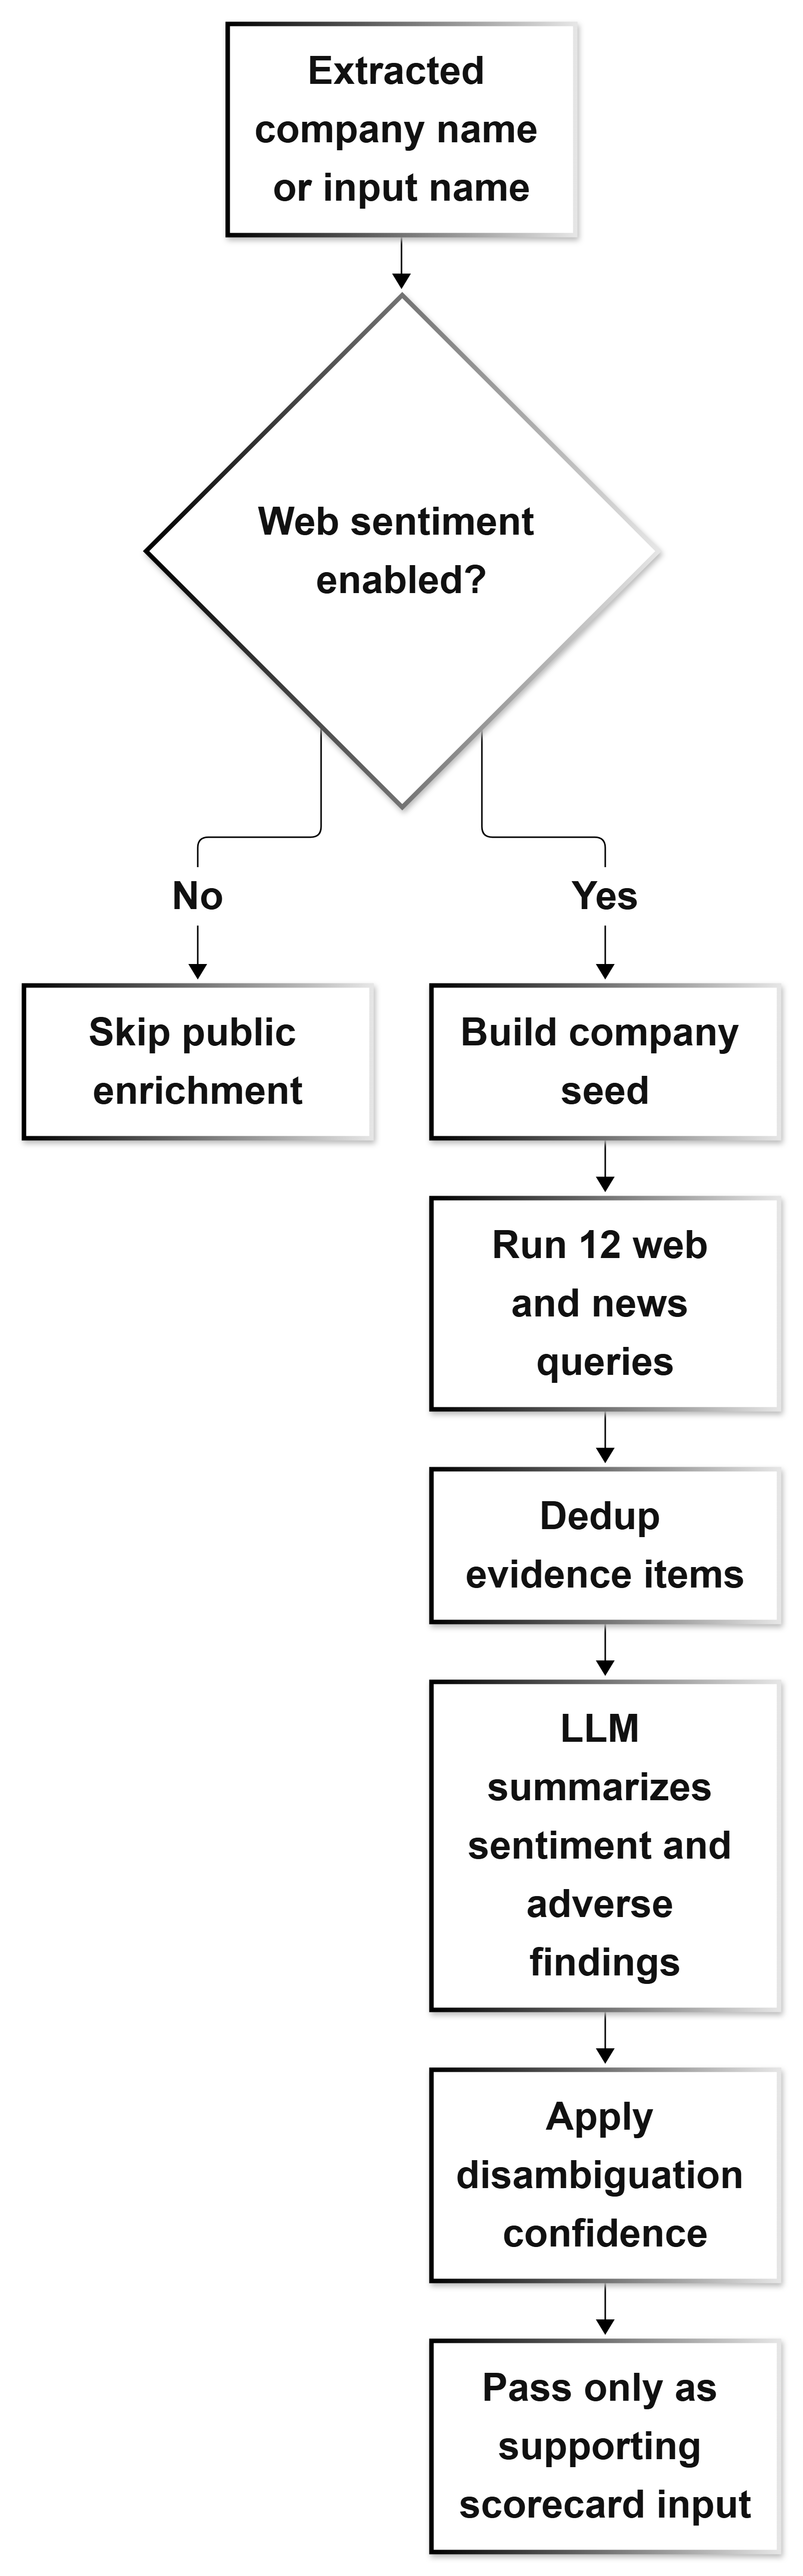
\includegraphics[width=\textwidth,height=0.85\textheight,keepaspectratio]{../diagrams/credit_risk/04_flowchart_optional-enrichment-flow.png}
\caption{Optional Enrichment Flow}
\label{fig:ch04_credit_risk-04-flowchart-optional-enrichment-flow}
\end{figure}
\speaker{Candidate}{With extraction and enrichment covered, can we go deeper into the deterministic ratio and scoring core next?}

\medskip\hrule\medskip
\section{Deterministic Financial Core}
\label{sec:ch04_credit_risk-6-deterministic-financial-core}

\speaker{Interviewer}{Now go deeper into the deterministic part. What exactly would Python compute?}

\speaker{Candidate}{Python would compute the full financial core.}

\subsection{Unit Normalization}

\begin{itemize}[leftmargin=\speakwid]
\item absolute = multiply by 1
\item thousands = multiply by 1,000
\item millions = multiply by 1,000,000
\end{itemize}
If duplicates exist for the same period and standardized label, I would aggregate or reconcile them carefully based on a clear aggregation policy.

\subsection{Derived Values}

\begin{itemize}[leftmargin=\speakwid]
\item EBITDA can be taken directly if present, else derived from EBIT plus depreciation and amortization when available.
\item Total debt can be taken directly if present, else derived from short-term debt plus long-term debt.
\end{itemize}
\subsection{Ratios}

\speaker{Candidate}{The system should compute a robust set of credit ratios, for example:}

\begin{itemize}[leftmargin=\speakwid]
\item Debt to equity.
\item Debt to assets.
\item Net debt to EBITDA.
\item Total liabilities to equity.
\item Current ratio.
\item Quick ratio.
\item Cash ratio.
\item EBITDA margin.
\item EBIT margin.
\item Net margin.
\item Return on equity.
\item Return on assets.
\item Return on capital employed.
\item Interest coverage.
\item DSCR.
\item OCF to total debt.
\item Cash conversion.
\item FCF margin.
\item Asset turnover.
\item Inventory days.
\item Days sales outstanding.
\end{itemize}
\speaker{Interviewer}{Why not let the LLM compute these directly if it already extracted the numbers?}

\speaker{Candidate}{Because deterministic functions are faster, cheaper, testable, and more reliable. In credit systems, the ratio formulas should be traceable and unit-tested. The LLM should explain the meaning of a ratio, not calculate it.}

\subsection{Deterministic Analytics Flow}

\begin{figure}[htbp]
\centering
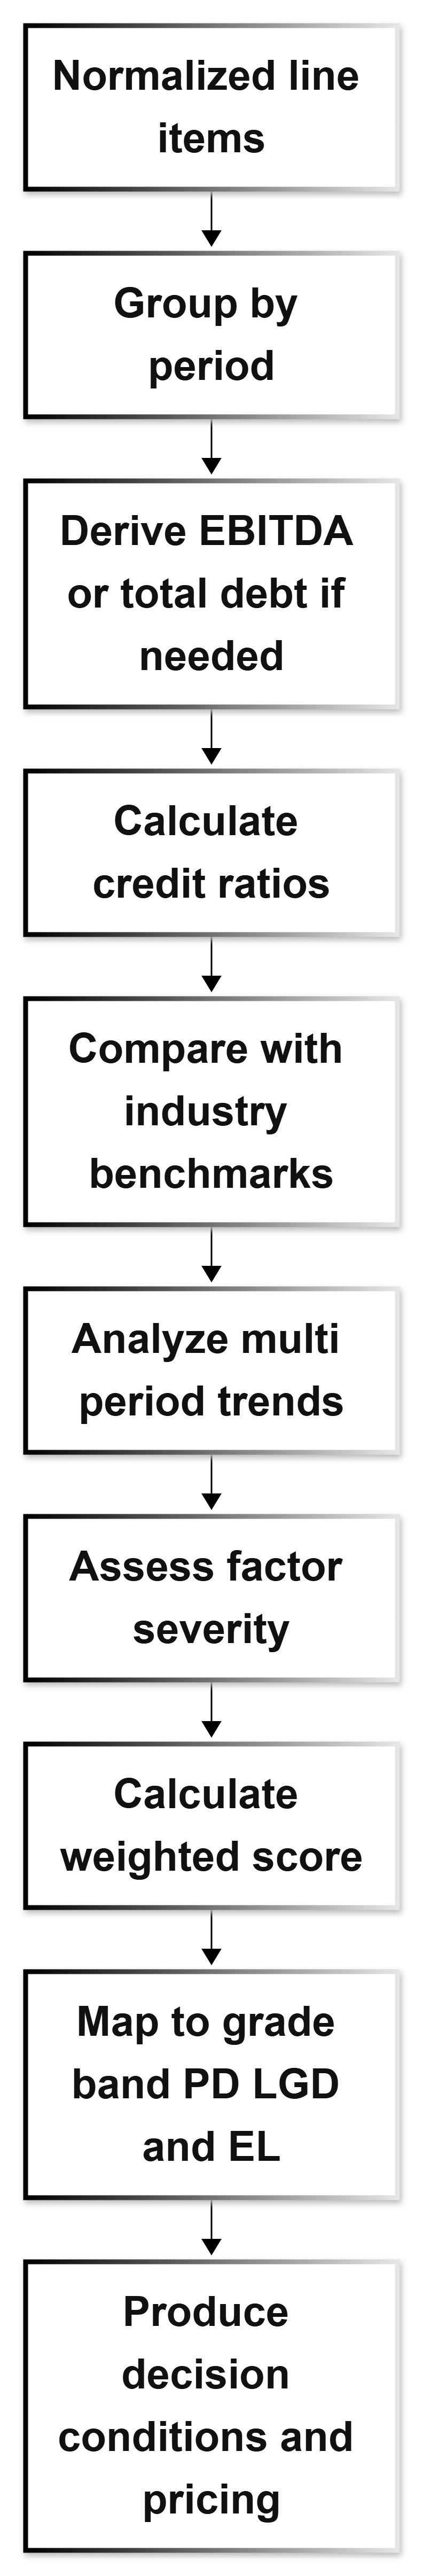
\includegraphics[width=\textwidth,height=0.85\textheight,keepaspectratio]{../diagrams/credit_risk/05_flowchart_deterministic-analytics-flow.png}
\caption{Deterministic Analytics Flow}
\label{fig:ch04_credit_risk-05-flowchart-deterministic-analytics-flow}
\end{figure}

\subsection{Benchmarks and Trends}

\speaker{Interviewer}{How do you use industry benchmarks?}

\speaker{Candidate}{Once the latest period ratios are computed, I would compare them against benchmark distributions such as median, lower quartile, and upper quartile for the relevant industry. This helps classify the borrower's relative position as strong, average, or weak and identify material gaps.}

\speaker{Interviewer}{And trends?}

\speaker{Candidate}{I would analyze whether key ratios are improving, stable, volatile, deteriorating, or mixed across time. This matters because a borrower with acceptable current ratios but sharply weakening trend may still be risky.}

\subsection{Scorecard}

\speaker{Interviewer}{Explain the scorecard logic. I want detail.}

\speaker{Candidate}{I would use a deterministic factor-based scorecard with defined weights and severity mapping. Example factor families include leverage, debt-service coverage, liquidity, profitability, cash-flow quality, deteriorating trend, sector underperformance, size and scale, audit quality, off-balance-sheet risk, adverse media, and market sentiment.}

\speakcont{Each factor gets:}

\begin{itemize}[leftmargin=\speakwid]
\item a weight,
\item a severity level such as low, medium, high, or critical,
\item a contribution to the normalized score,
\item evidence text,
\item and sometimes related pages.
\end{itemize}
\speakcont{Then the aggregate score maps to grade, risk band, PD, LGD, expected loss, decision, and conditions.}

\speaker{Interviewer}{Why do you prefer a factor scorecard instead of a black-box ML model?}

\speaker{Candidate}{Because the business requirement here strongly favors interpretability, reproducibility, and policy alignment. Analysts need to understand why the system recommends a result. A factor scorecard also aligns well with memo writing because the risk drivers are already explicit.}

\speaker{Interviewer}{Give me the actual numbers behind that scorecard. Weights, thresholds, and how the score becomes a grade and a decision.}

\speaker{Candidate}{Happy to, because the numbers are the business policy. The thirteen factor weights are leverage 22, debt-service coverage 22, liquidity 16, profitability 16, cash-flow quality 14, deteriorating trend 16, sector underperformance 10, size and scale 8, jurisdiction 6, audit quality 20, off-balance-sheet 10, adverse media 14, and market sentiment 8. Severity multiplies the weight: low by 0.0, medium by 0.6, high by 1.0, and critical by 1.6, rounded to two decimals, and anything above low counts as present. Key thresholds are net debt to EBITDA at 3.0, 4.5, and 6.0; interest cover at 4.0, 2.0, and 1.0; DSCR at 1.5, 1.2, and 1.0; current ratio at 1.2, 1.0, and 0.8; EBITDA margin at 0.10, 0.05, and 0.0; and cash conversion at 0.8, 0.5, and 0.2. Size uses unit-normalised latest revenue with 10 million as medium and 2 million as high. Coverage takes the worse of interest cover and DSCR, and a deteriorating significant trend on a core ratio pushes the trend factor high. The raw sum is capped at 100, and a hard stop forces 100. Grades map from max score as 5 AAA, 12 AA, 20 A, 32 BBB, 45 BB, 60 B, 75 CCC, 88 CC, 97 C, and 100 D, with bands from investment-grade-strong down to default. PD follows the grade from 0.0001 for AAA up to 1.0 for D, LGD follows industry at 0.40 manufacturing, 0.45 retail and general, and 0.55 services, and expected loss is PD times LGD rounded to six decimals. Hard-stop, default, or distressed means decline; speculative means refer to the credit committee; sub-investment or any material gap means approve with conditions; otherwise approve. Conditions and pricing follow the band, for example leverage covenants, minimum DSCR, liquidity floors, cash sweeps, guarantee caps, collateral, and spreads from plus 80--130 basis points when strong up to bespoke secured-only when distressed. So every memo sentence about leverage or coverage traces back to one of these exact cutoffs.}

\subsection{Scorecard Decision Sequence}

\begin{figure}[htbp]
\centering
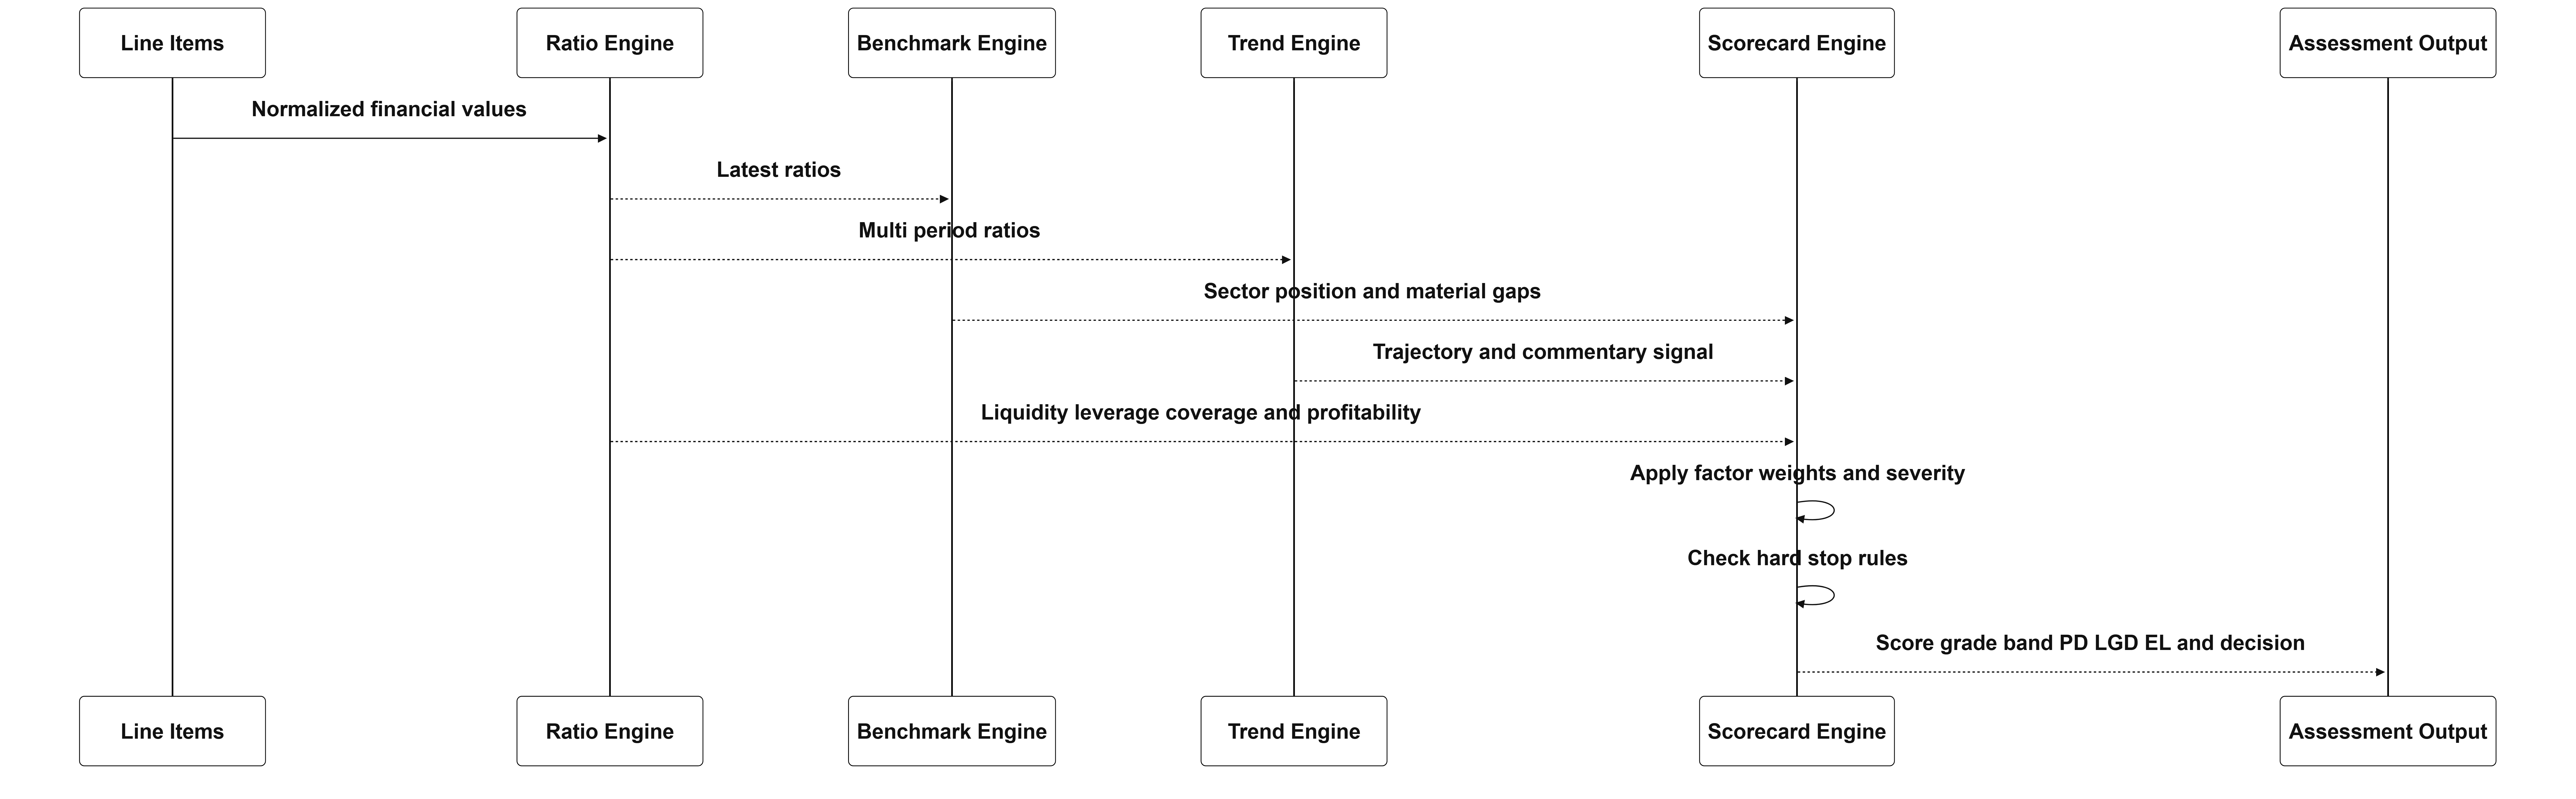
\includegraphics[width=\textwidth,height=0.85\textheight,keepaspectratio]{../diagrams/credit_risk/06_sequenceDiagram_scorecard-decision-sequence.png}
\caption{Scorecard Decision Sequence}
\label{fig:ch04_credit_risk-06-sequencediagram-scorecard-decision-sequence}
\end{figure}

\subsection{Hard Stops}

\speaker{Interviewer}{What kinds of cases should trigger a hard stop?}

\speaker{Candidate}{At minimum, situations like adverse or disclaimer audit opinion, or explicit going-concern uncertainty in the notes. These are serious enough that the system should not present a normal approval-style recommendation path.}

\speaker{Interviewer}{Would the hard stop bypass the memo?}

\speaker{Candidate}{No, I would still draft the memo, but the memo should clearly reflect the hard-stop reason and proposed decline path. The human approver still reviews it.}
\speaker{Candidate}{With ratios, benchmarks, and the scorecard settled, shall we cover how the draft memo is generated from those results?}

\medskip\hrule\medskip
\section{Memo Generation and Q\&A}
\label{sec:ch04_credit_risk-7-memo-generation-and-q-a}

\speaker{Interviewer}{Now explain the memo generation part. How do you use the LLM safely there?}

\speaker{Candidate}{I would never ask the memo model to read raw PDFs directly in the final stage. Instead, I would feed it a compact JSON generated by the deterministic pipeline. That JSON would include company metadata, facility summary, computed ratios, scorecard, active factors, trend summary, benchmark summary, off-balance-sheet items, and optional web sentiment summary.}

\speaker{Interviewer}{Why is that safer?}

\speaker{Candidate}{Because it narrows the LLM's job to narration, structuring, and explanation. The memo model is not discovering numbers; it is writing about already-computed results. That reduces hallucination and keeps the memo aligned with the scorecard.}

\speaker{Interviewer}{What should the memo contain?}

\speaker{Candidate}{At least:}

\begin{itemize}[leftmargin=\speakwid]
\item Executive summary.
\item Financial analysis.
\item Key strengths.
\item Key risks.
\item Mitigants.
\item Recommended covenants.
\item Monitoring triggers.
\end{itemize}
\speaker{Interviewer}{Can the user ask follow-up questions after the memo is generated?}

\speaker{Candidate}{Yes. I would support a Q\&A endpoint that answers only from the completed assessment JSON. It should never invent a new grade, a new ratio, or a different decision. If the answer is not present in the assessment, it should say so clearly.}

\subsection{Memo Generation Flow}

\begin{figure}[htbp]
\centering
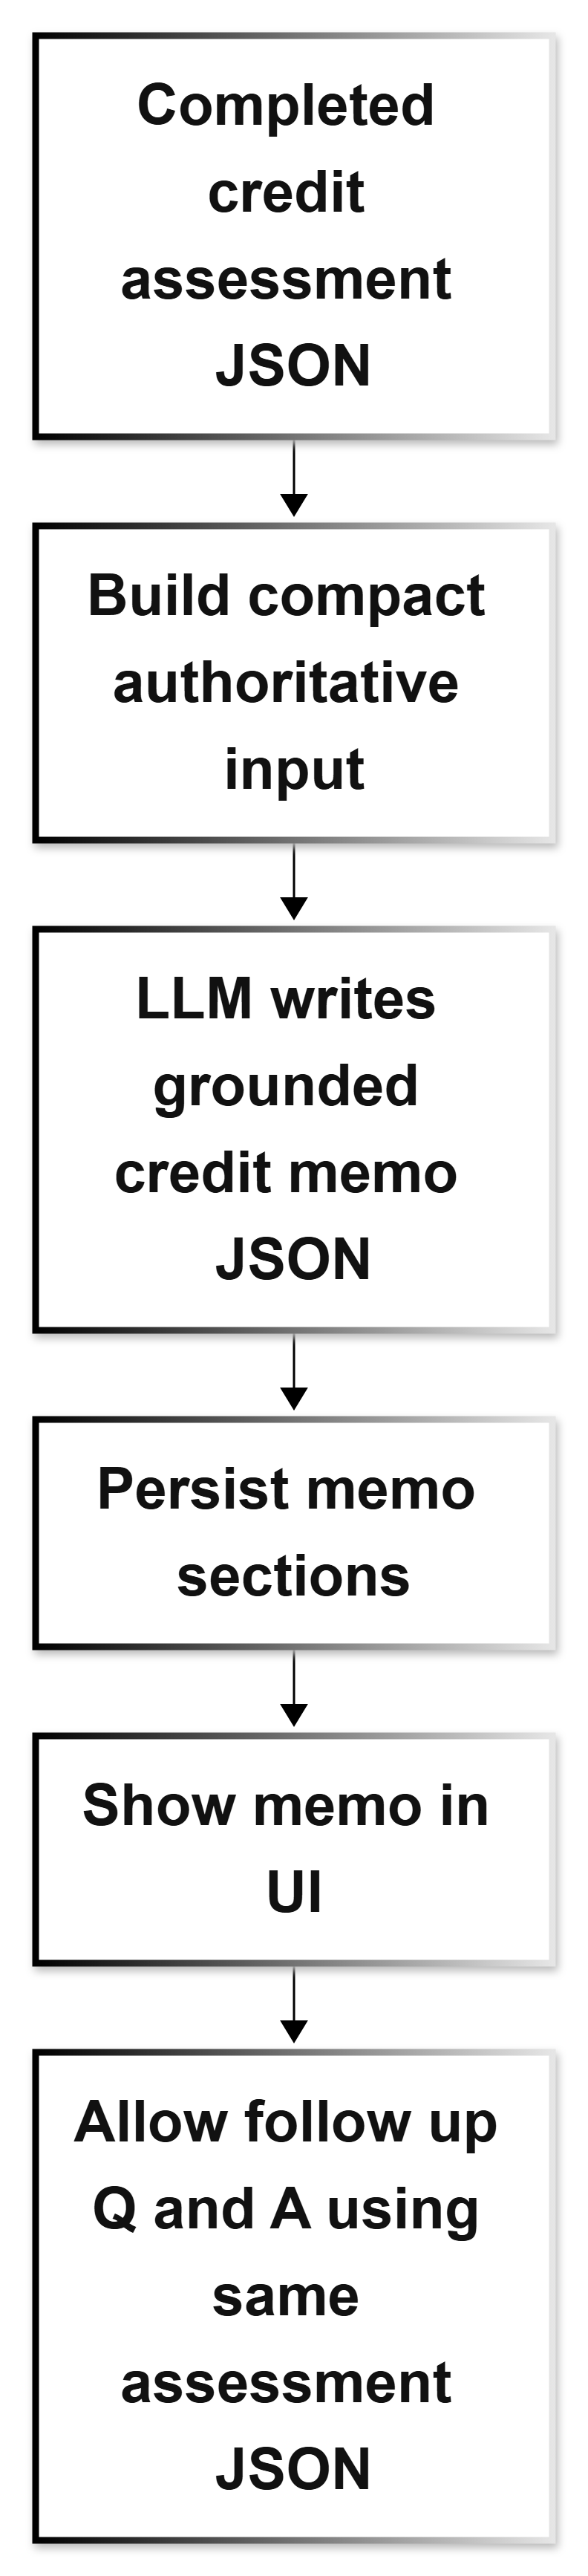
\includegraphics[width=\textwidth,height=0.85\textheight,keepaspectratio]{../diagrams/credit_risk/07_flowchart_memo-generation-flow.png}
\caption{Memo Generation Flow}
\label{fig:ch04_credit_risk-07-flowchart-memo-generation-flow}
\end{figure}
\speaker{Candidate}{With the memo and Q\&A flow clear, can we step back to the high-level system architecture next?}

\medskip\hrule\medskip
\section{High-Level Design}
\label{sec:ch04_credit_risk-8-high-level-design}

\speaker{Interviewer}{Great. Please describe the high-level system architecture.}

\speaker{Candidate}{At a high level, I would keep the design simple and production-oriented.}

\subsection{Architecture Components}

\begin{enumerate}[leftmargin=\speakwid]
\item Thin client UI, such as Streamlit or a small web frontend.
\item FastAPI backend exposing assessment, status, review, question, rerun, and audit endpoints.
\item S3 or ADLS object storage for documents.
\item Postgres as the source of truth for versions, documents, page chunks, line items, ratios, factors, memos, and reviews.
\item pgvector inside Postgres for page embeddings and semantic search.
\item Redis for ephemeral live phase tracking.
\item LLM gateway for extraction, sentiment summarization, memo generation, and Q\&A.
\item Optional yfinance and DuckDuckGo-based enrichment modules.
\item Deterministic Python services for ratios, benchmarks, trend analysis, and scoring.
\end{enumerate}
\subsection{High-Level Architecture Diagram}

\begin{figure}[htbp]
\centering
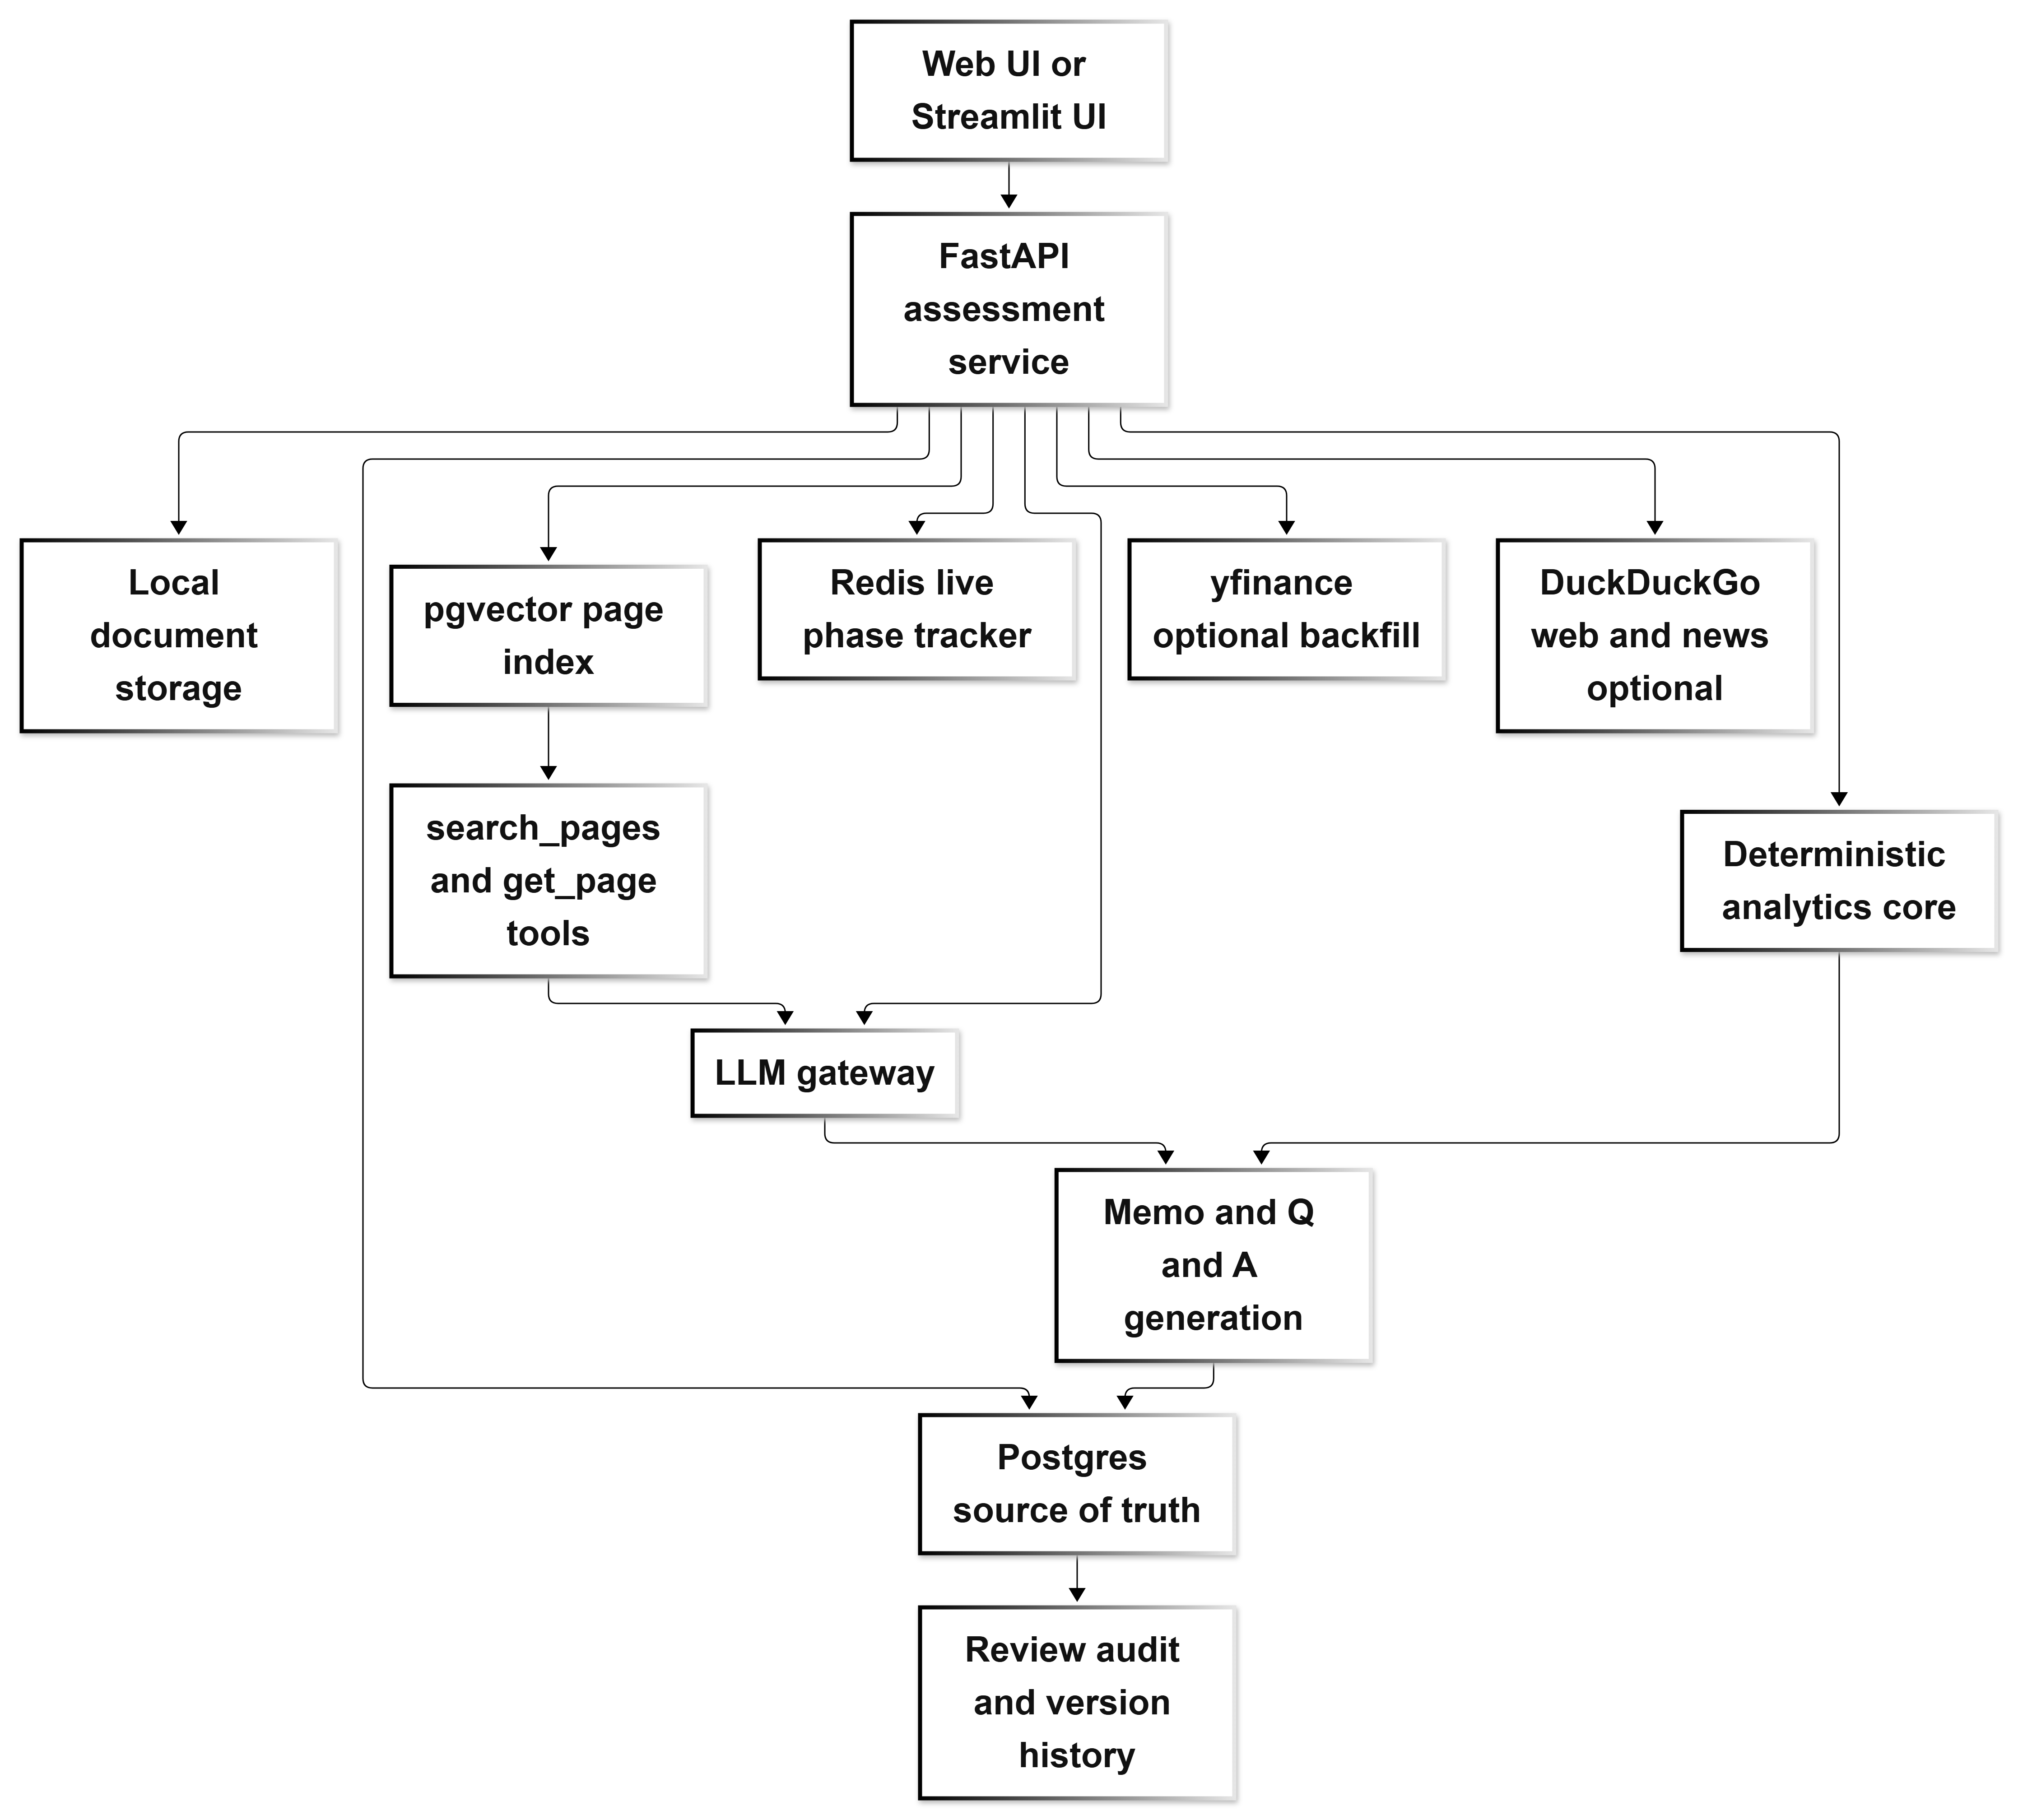
\includegraphics[width=\textwidth,height=0.85\textheight,keepaspectratio]{../diagrams/credit_risk/08_flowchart_high-level-architecture-diagram.png}
\caption{High-Level Architecture Diagram}
\label{fig:ch04_credit_risk-08-flowchart-high-level-architecture-diagram}
\end{figure}

\speaker{Interviewer}{Why keep it as one service instead of splitting it now?}

\speaker{Candidate}{Because the design goals here are clarity, traceability, and reproducibility. The workflow is sequential and tightly coupled around one assessment version. Splitting it too early would add operational complexity without much benefit.}
\speaker{Candidate}{With the high-level shape agreed, shall we dive into the low-level request lifecycle and review-rerun handling?}

\medskip\hrule\medskip
\section{Low-Level Design}
\label{sec:ch04_credit_risk-9-low-level-design}

\speaker{Interviewer}{Now go into low-level design. I want more than a box diagram.}

\speaker{Candidate}{Sure. I would define the low-level design around a version-centric workflow.}

\subsection{Request Lifecycle}

\begin{itemize}[leftmargin=\speakwid]
\item \texttt{POST /assessments} accepts multipart form-data.
\item Files are uploaded to an S3 or ADLS prefix for the request.
\item A new \texttt{assessment\_version} row is created with status \texttt{created}.
\item Redis phase is set to \texttt{queued}.
\item Background processing starts.
\item Final results are written, then status becomes \texttt{awaiting\_review}.
\end{itemize}
\subsection{Core Application Modules}

\begin{itemize}[leftmargin=\speakwid]
\item \texttt{api/main.py} for app bootstrapping and schema initialization.
\item \texttt{api/routes.py} for endpoints and background-task kickoff.
\item \texttt{doc\_index.py} for PDF-to-page extraction.
\item \texttt{db/page\_index.py} for pgvector ingest and retrieval.
\item \texttt{tools.py} and \texttt{tool\_loop.py} for bounded tool calling.
\item \texttt{extraction.py} for structured extraction agents.
\item \texttt{ratios.py}, \texttt{benchmarks.py}, \texttt{scoring.py} for deterministic logic.
\item \texttt{marketdata.py} and \texttt{osint/*} for optional enrichment.
\item \texttt{narrative.py} for memo synthesis.
\item \texttt{db/persist.py} for structured writes.
\end{itemize}
\subsection{Tool Loop Behavior}

\speaker{Interviewer}{How exactly should the tool loop behave?}

\speaker{Candidate}{The loop should bind the available tools to the LLM, execute requested tool calls, append tool outputs into the message history, and repeat until the model returns a final JSON answer or the maximum iteration limit is reached. Unknown tools or tool errors should be returned to the model as tool messages, not hidden.}

\speaker{Candidate}{Can I also spell out the API contract and the two supporting modules that make this loop production-usable, since the endpoints are where the business workflow meets the system?}

\speaker{Interviewer}{Yes. Which endpoints and modules matter most?}

\speaker{Candidate}{There are eight REST endpoints. Health returns ok. Listing returns version summaries newest first. Creating accepts multipart files plus company name, ticker, question, search region, web-sentiment flag, and requester, then returns 202 with the version id. Fetching returns the full assessment response with summary fields, PD, LGD, expected loss, hard-stop reason, latency, LLM call count, model names, the raw assessment JSON, reasoning list, and document names. Status returns the version id, Postgres status, and the Redis phase. Rerun accepts an instruction JSON and returns a new version. Question accepts a question string and returns the answer, with 409 if the run is not finished. Review accepts reviewer, action, corrected fields, and reason. Audit returns the version, parent link, documents with hash and page count, line items with label and page, rating factors with severity and evidence, and reviews. Bad ids give 404. Two modules deserve attention. The correctness gate in \texttt{llm\_validation.py} adds the confidence scoring and bounded retry I described earlier, and \texttt{review\_feedback.py} consumes the review rows through \texttt{get\_review\_history()} and \texttt{apply\_review\_corrections()} for audit display. Configuration pins the LLM model name, temperature 0.0, max tokens 4096, embedding dimension 1536, yfinance discrepancy tolerance 0.02, OSINT region, result limit and timeout, a Redis phase TTL of 3600 seconds, and four parallel extractor workers. The per-run LLM call count follows four calls when PDFs exist plus one memo call plus one web call when enrichment runs plus one per follow-up question.}

\subsection{Failure Handling}

\speaker{Interviewer}{What if one extraction step fails?}

\speaker{Candidate}{I would distinguish between optional and critical failures.}

\begin{itemize}[leftmargin=\speakwid]
\item If yfinance fails, skip it.
\item If web sentiment fails, skip it.
\item If one of the core extractors or downstream deterministic scoring fails, move the case to \texttt{validation\_review} instead of pretending the output is complete.
\end{itemize}
\speakcont{This preserves partial evidence such as uploaded documents and page chunks but avoids writing a misleading final scorecard.}

\subsection{Atomic Persistence}

\speaker{Interviewer}{Why does atomic persistence matter here?}

\speaker{Candidate}{Because half-written credit decisions are dangerous. I would persist line items, ratios, rating factors, memo, and final version update in one transaction so that the system never shows a completed result with missing internal components.}

\subsection{Review and Rerun}

\speaker{Interviewer}{How would corrected reviews work?}

\speaker{Candidate}{A review action can be approved, corrected, or rejected. Corrections should be stored as review records with corrected fields and reason. If a new run is required, rerun should create a new version linked to the parent version rather than mutating history. That keeps a clean audit trail.}

\subsection{Review and Rerun Sequence}

\begin{figure}[htbp]
\centering
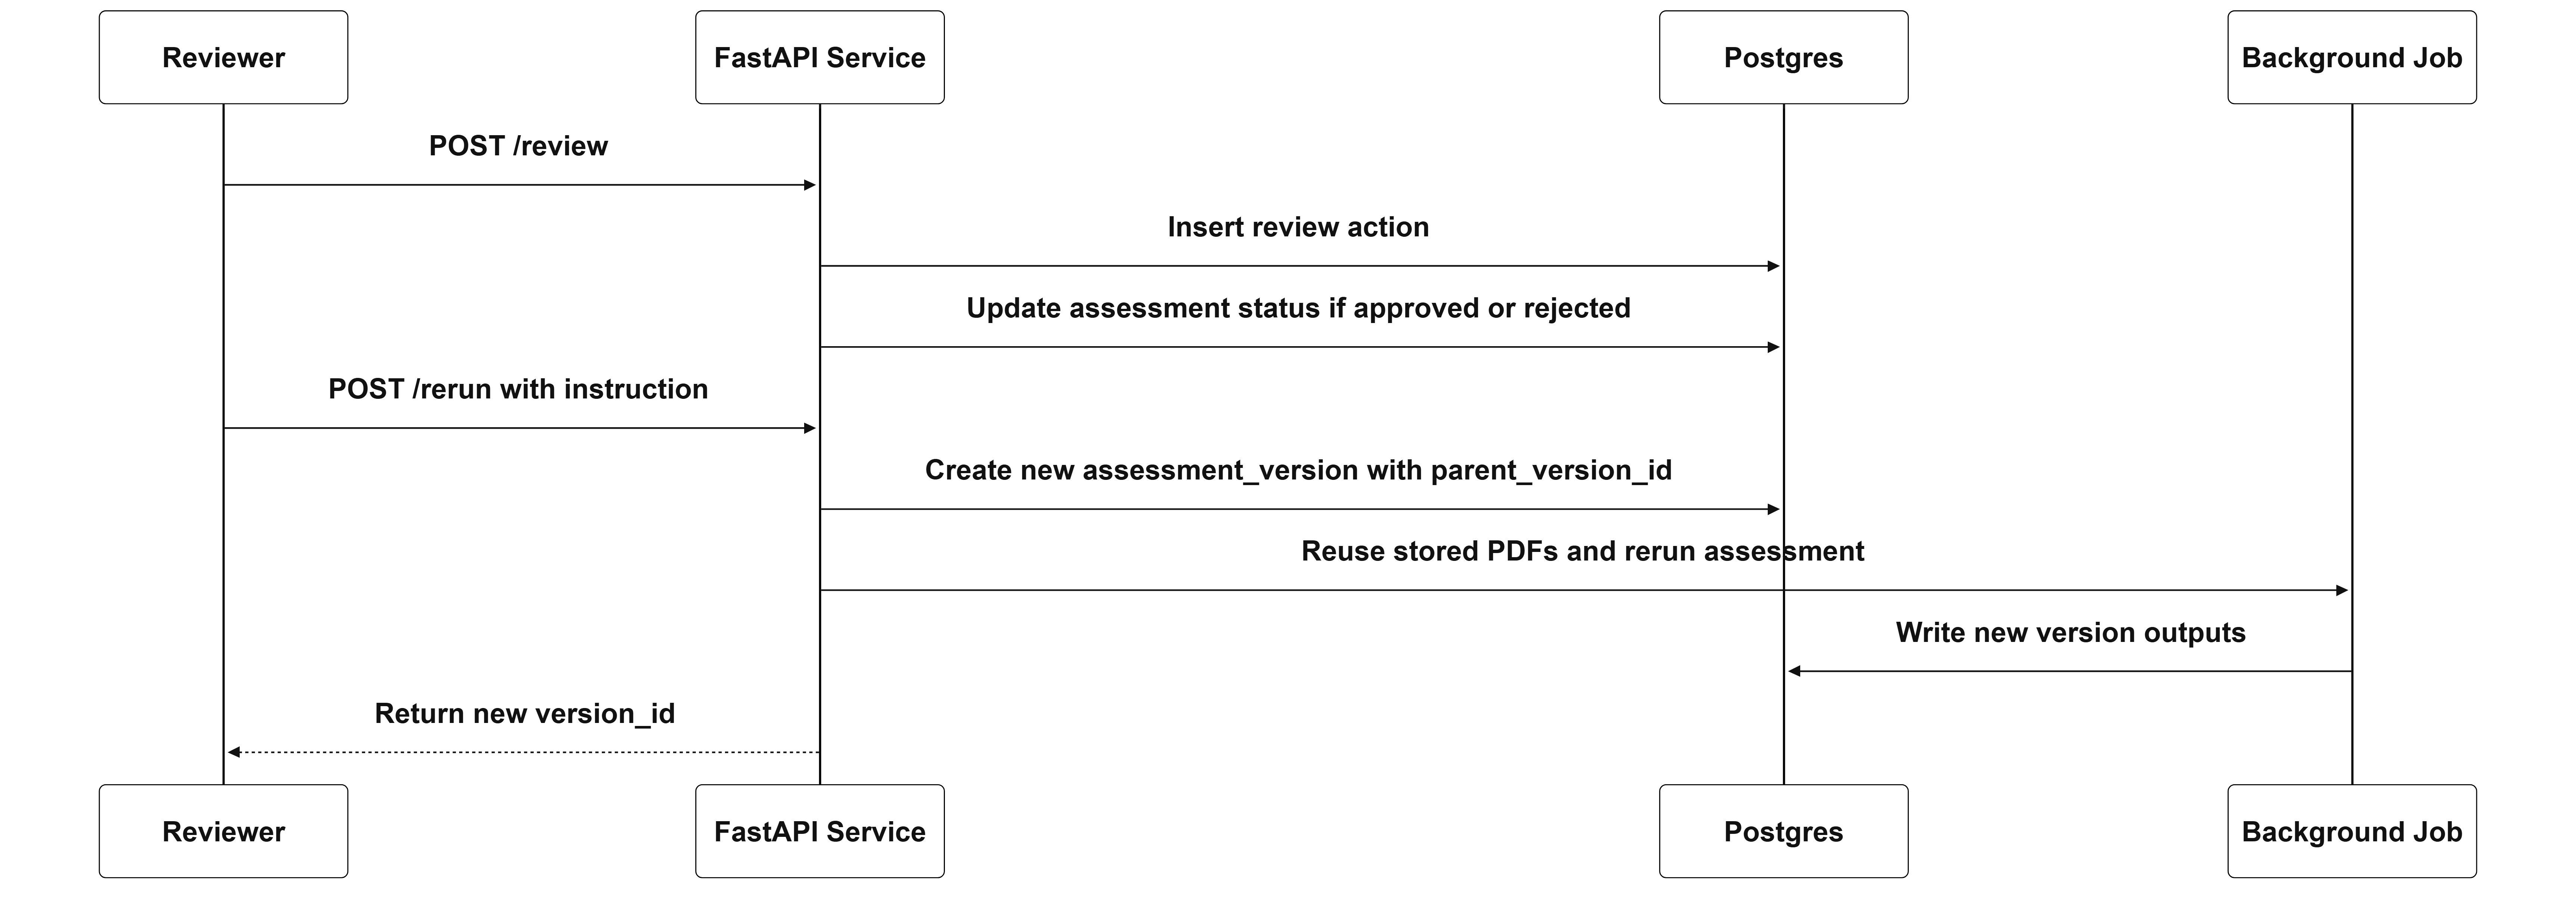
\includegraphics[width=\textwidth,height=0.85\textheight,keepaspectratio]{../diagrams/credit_risk/09_sequenceDiagram_review-and-rerun-sequence.png}
\caption{Review and Rerun Sequence}
\label{fig:ch04_credit_risk-09-sequencediagram-review-and-rerun-sequence}
\end{figure}
\speaker{Candidate}{With the request and review flow clear, can we detail the versioned data model and audit lineage next?}

\medskip\hrule\medskip
\section{Data Modeling}
\label{sec:ch04_credit_risk-10-data-modeling}

\speaker{Interviewer}{Good. Now I want the data modeling section in detail. Include the entity relationship diagram and the tables.}

\speaker{Candidate}{Sure. The most important design choice is to make the assessment version the anchor entity. Every major result object should connect to the version. That prevents ambiguous joins and makes audit and rerun lineage straightforward.}

\subsection{Entity Relationship Diagram}

\begin{figure}[htbp]
\centering
\includegraphics[width=\textwidth,height=0.85\textheight,keepaspectratio]{../diagrams/credit_risk/10_erDiagram_10-1-entity-relationship-diagram.png}
\caption{Entity Relationship Diagram}
\label{fig:ch04_credit_risk-10-erdiagram-10-1-entity-relationship-diagram}
\end{figure}

\subsection{Join Paths Readers Should Remember}

\begin{xltabular}{\textwidth}{>{\raggedright\arraybackslash}X >{\raggedright\arraybackslash}X >{\raggedright\arraybackslash}X >{\raggedright\arraybackslash}X}
\caption{Join Paths Readers Should Remember}\label{tab:ch04_credit_risk-10-2-join-paths-readers-should-remember-1}\\
\hline
\textbf{From Table} & \textbf{To Table} & \textbf{Join Condition} & \textbf{Why the Join Matters} \\
\hline
\endfirsthead
\caption[]{Join Paths Readers Should Remember (continued)}\\
\hline
\textbf{From Table} & \textbf{To Table} & \textbf{Join Condition} & \textbf{Why the Join Matters} \\
\hline
\endhead
\texttt{assessment\_versions} & \texttt{assessment\_documents} & \texttt{assessment\_versions.id = assessment\_documents.assessment\_version\_id} & Find all uploaded documents for one run \\
\texttt{assessment\_documents} & \texttt{page\_chunks} & \texttt{assessment\_documents.id = page\_chunks.document\_id} & Trace a page back to its source file \\
\texttt{assessment\_versions} & \texttt{page\_chunks} & \texttt{assessment\_versions.id = page\_chunks.\allowbreak{}assessment\_version\_id} & Fetch all indexed pages for a run \\
\texttt{assessment\_versions} & \texttt{line\_items} & \texttt{assessment\_versions.id = line\_items.assessment\_version\_id} & Get structured extracted values for a run \\
\texttt{assessment\_versions} & \texttt{ratios} & \texttt{assessment\_versions.id = ratios.assessment\_version\_id} & Load calculated ratios for a run \\
\texttt{assessment\_versions} & \texttt{rating\_factors} & \texttt{assessment\_versions.id = rating\_factors.assessment\_version\_id} & Explain why the score was assigned \\
\texttt{assessment\_versions} & \texttt{credit\_memos} & \texttt{assessment\_versions.id = credit\_memos.assessment\_version\_id} & Retrieve memo text for the run \\
\texttt{assessment\_versions} & \texttt{reviews} & \texttt{assessment\_versions.id = reviews.assessment\_version\_id} & Show reviewer decisions and corrections \\
\texttt{assessment\_versions} & \texttt{assessment\_versions} & \texttt{child.parent\_version\_id = parent.id} & Traverse rerun lineage \\
\hline
\end{xltabular}

\subsection{Physical Table Structures}

\subsubsection{Table: \texttt{assessment\_versions}}

\begin{xltabular}{\textwidth}{>{\raggedright\arraybackslash}X >{\raggedright\arraybackslash}X >{\raggedright\arraybackslash}X >{\raggedright\arraybackslash}X >{\raggedright\arraybackslash}X}
\caption{Table: assessment\_versions}\label{tab:ch04_credit_risk-table-assessment-versions-2}\\
\hline
\textbf{Column Name} & \textbf{Data Type} & \textbf{PK/FK} & \textbf{Nullable} & \textbf{Description} \\
\hline
\endfirsthead
\caption[]{Table: assessment\_versions (continued)}\\
\hline
\textbf{Column Name} & \textbf{Data Type} & \textbf{PK/FK} & \textbf{Nullable} & \textbf{Description} \\
\hline
\endhead
\texttt{id} & UUID & PK & No & Unique id for this assessment run \\
\texttt{parent\_version\_id} & UUID & FK -> \texttt{assessment\_versions.id} & Yes & Links rerun to parent version \\
\texttt{status} & VARCHAR(32) & - & No & \texttt{created}, \texttt{processing}, \texttt{awaiting\_review}, \texttt{validation\_review}, \texttt{approved}, \texttt{rejected} \\
\texttt{company\_name} & VARCHAR(255) & - & Yes & Input or resolved borrower name \\
\texttt{ticker} & VARCHAR(16) & - & Yes & Optional market ticker \\
\texttt{question} & TEXT & - & Yes & Optional initial question \\
\texttt{instruction} & TEXT & - & Yes & Optional rerun instruction \\
\texttt{answer} & TEXT & - & Yes & Latest follow-up answer \\
\texttt{enable\_web\_sentiment} & BOOLEAN & - & No & Whether public web enrichment is enabled \\
\texttt{search\_region} & VARCHAR(16) & - & Yes & Region hint for web search \\
\texttt{model\_name} & VARCHAR(128) & - & Yes & LLM model used \\
\texttt{embed\_model\_name} & VARCHAR(128) & - & Yes & Embedding model used \\
\texttt{grade} & VARCHAR(8) & - & Yes & Final rating grade \\
\texttt{band} & VARCHAR(32) & - & Yes & Final risk band \\
\texttt{decision} & VARCHAR(32) & - & Yes & Proposed decision \\
\texttt{probability\_of\_default} & FLOAT & - & Yes & PD from deterministic mapping \\
\texttt{loss\_given\_default} & FLOAT & - & Yes & LGD by industry/table \\
\texttt{expected\_loss\_pct} & FLOAT & - & Yes & Expected loss percent \\
\texttt{hard\_stop\_reason} & TEXT & - & Yes & Reason if hard-stop logic triggered \\
\texttt{latency\_ms} & FLOAT & - & Yes & End-to-end runtime \\
\texttt{llm\_call\_count} & INTEGER & - & Yes & Count of LLM calls in the run \\
\texttt{raw\_result} & JSONB & - & Yes & Full serialized credit assessment \\
\texttt{reasoning} & JSONB & - & Yes & Structured reasoning list \\
\texttt{requested\_by} & VARCHAR(128) & - & No & Analyst or caller id \\
\texttt{requested\_at} & TIMESTAMP\-TZ & - & No & Request creation timestamp \\
\texttt{completed\_at} & TIMESTAMP\-TZ & - & Yes & Run completion timestamp \\
\hline
\end{xltabular}

\subsubsection{Table: \texttt{assessment\_documents}}

\begin{xltabular}{\textwidth}{>{\raggedright\arraybackslash}X >{\raggedright\arraybackslash}X >{\raggedright\arraybackslash}X >{\raggedright\arraybackslash}X >{\raggedright\arraybackslash}X}
\caption{Table: assessment\_documents}\label{tab:ch04_credit_risk-table-assessment-documents-3}\\
\hline
\textbf{Column Name} & \textbf{Data Type} & \textbf{PK/FK} & \textbf{Nullable} & \textbf{Description} \\
\hline
\endfirsthead
\caption[]{Table: assessment\_documents (continued)}\\
\hline
\textbf{Column Name} & \textbf{Data Type} & \textbf{PK/FK} & \textbf{Nullable} & \textbf{Description} \\
\hline
\endhead
\texttt{id} & UUID & PK & No & Unique document row id \\
\texttt{assessment\_version\_id} & UUID & FK -> \texttt{assessment\_versions.id} & No & Owning assessment version \\
\texttt{filename} & VARCHAR(255) & - & No & Original uploaded filename \\
\texttt{storage\_uri} & TEXT & - & No & Absolute or object-storage path \\
\texttt{sha256\_hash} & VARCHAR(64) & - & No & File hash for integrity \\
\texttt{page\_count} & INTEGER & - & No & Number of pages in the document \\
\hline
\end{xltabular}

\subsubsection{Table: \texttt{page\_chunks}}

\begin{xltabular}{\textwidth}{>{\raggedright\arraybackslash}X >{\raggedright\arraybackslash}X >{\raggedright\arraybackslash}X >{\raggedright\arraybackslash}X >{\raggedright\arraybackslash}X}
\caption{Table: page\_chunks}\label{tab:ch04_credit_risk-table-page-chunks-4}\\
\hline
\textbf{Column Name} & \textbf{Data Type} & \textbf{PK/FK} & \textbf{Nullable} & \textbf{Description} \\
\hline
\endfirsthead
\caption[]{Table: page\_chunks (continued)}\\
\hline
\textbf{Column Name} & \textbf{Data Type} & \textbf{PK/FK} & \textbf{Nullable} & \textbf{Description} \\
\hline
\endhead
\texttt{id} & UUID & PK & No & Unique page chunk id \\
\texttt{assessment\_version\_id} & UUID & FK -> \texttt{assessment\_versions.id} & No & Assessment to which page belongs \\
\texttt{document\_id} & UUID & FK -> \texttt{assessment\_documents.id} & Yes & Source document row \\
\texttt{page\_number} & INTEGER & - & No & Global page number across pack \\
\texttt{doc\_name} & VARCHAR(255) & - & No & Human-readable file name \\
\texttt{text} & TEXT & - & No & Full extracted text for that page \\
\texttt{embedding} & VECTOR & - & Yes & pgvector embedding for semantic search \\
\hline
\end{xltabular}

\subsubsection{Table: \texttt{line\_items}}

\begin{xltabular}{\textwidth}{>{\raggedright\arraybackslash}X >{\raggedright\arraybackslash}X >{\raggedright\arraybackslash}X >{\raggedright\arraybackslash}X >{\raggedright\arraybackslash}X}
\caption{Table: line\_items}\label{tab:ch04_credit_risk-table-line-items-5}\\
\hline
\textbf{Column Name} & \textbf{Data Type} & \textbf{PK/FK} & \textbf{Nullable} & \textbf{Description} \\
\hline
\endfirsthead
\caption[]{Table: line\_items (continued)}\\
\hline
\textbf{Column Name} & \textbf{Data Type} & \textbf{PK/FK} & \textbf{Nullable} & \textbf{Description} \\
\hline
\endhead
\texttt{id} & UUID & PK & No & Unique line item id \\
\texttt{assessment\_version\_id} & UUID & FK -> \texttt{assessment\_versions.id} & No & Owning assessment version \\
\texttt{label} & VARCHAR(255) & - & No & Raw label from statement \\
\texttt{standardised\_label} & VARCHAR(64) & - & No & Controlled vocabulary label \\
\texttt{value} & FLOAT & - & Yes & Numeric value after parsing \\
\texttt{currency} & VARCHAR(16) & - & Yes & Currency code or symbol \\
\texttt{unit} & VARCHAR(16) & - & No & \texttt{absolute}, \texttt{thousands}, \texttt{millions} \\
\texttt{period} & VARCHAR(32) & - & No & Logical period label such as FY2023 \\
\texttt{statement\_type} & VARCHAR(32) & - & No & Balance sheet, income statement, cash flow, notes, other \\
\texttt{page} & INTEGER & - & Yes & Source page number \\
\texttt{source\_snippet} & TEXT & - & Yes & Small source snippet or origin tag \\
\hline
\end{xltabular}

\speaker{Interviewer}{Your line-items table looks slightly simplified. What period fields should we persist?}

\speaker{Candidate}{Good catch. Beyond label, value, currency, unit, period, statement type, page, and snippet, each line-item row also carries \texttt{period\_type} such as annual, interim, or quarterly, an ISO \texttt{period\_end\_date} when stated, and \texttt{period\_length\_months} in values like 12, 6, 3, or 9. For the business workflow those three fields matter: they let Python separate audited annuals from interim management accounts, order periods by year for trend analysis, and avoid annualising a half-year figure as if it were a full year. That is why the extractor prompt forces one record per item per period with a consistent period string across statements.}

\subsubsection{Table: \texttt{ratios}}

\begin{xltabular}{\textwidth}{>{\raggedright\arraybackslash}X >{\raggedright\arraybackslash}X >{\raggedright\arraybackslash}X >{\raggedright\arraybackslash}X >{\raggedright\arraybackslash}X}
\caption{Table: ratios}\label{tab:ch04_credit_risk-table-ratios-6}\\
\hline
\textbf{Column Name} & \textbf{Data Type} & \textbf{PK/FK} & \textbf{Nullable} & \textbf{Description} \\
\hline
\endfirsthead
\caption[]{Table: ratios (continued)}\\
\hline
\textbf{Column Name} & \textbf{Data Type} & \textbf{PK/FK} & \textbf{Nullable} & \textbf{Description} \\
\hline
\endhead
\texttt{id} & UUID & PK & No & Unique ratio row id \\
\texttt{assessment\_version\_id} & UUID & FK -> \texttt{assessment\_versions.id} & No & Owning assessment version \\
\texttt{period} & VARCHAR(32) & - & No & Ratio period \\
\texttt{ratio\_name} & VARCHAR(64) & - & No & Name such as \texttt{current\_ratio}, \texttt{dscr} \\
\texttt{value} & FLOAT & - & Yes & Ratio value \\
\texttt{category} & VARCHAR(32) & - & No & Liquidity, leverage, coverage, etc. \\
\texttt{inputs\_used} & JSONB & - & Yes & Financial labels used to compute ratio \\
\texttt{missing\_inputs} & JSONB & - & Yes & Missing labels if ratio could not be computed \\
\texttt{pages} & JSONB & - & Yes & Related source pages \\
\hline
\end{xltabular}

\subsubsection{Table: \texttt{rating\_factors}}

\begin{xltabular}{\textwidth}{>{\raggedright\arraybackslash}X >{\raggedright\arraybackslash}X >{\raggedright\arraybackslash}X >{\raggedright\arraybackslash}X >{\raggedright\arraybackslash}X}
\caption{Table: rating\_factors}\label{tab:ch04_credit_risk-table-rating-factors-7}\\
\hline
\textbf{Column Name} & \textbf{Data Type} & \textbf{PK/FK} & \textbf{Nullable} & \textbf{Description} \\
\hline
\endfirsthead
\caption[]{Table: rating\_factors (continued)}\\
\hline
\textbf{Column Name} & \textbf{Data Type} & \textbf{PK/FK} & \textbf{Nullable} & \textbf{Description} \\
\hline
\endhead
\texttt{id} & UUID & PK & No & Unique factor row id \\
\texttt{assessment\_version\_id} & UUID & FK -> \texttt{assessment\_versions.id} & No & Owning assessment version \\
\texttt{factor\_type} & VARCHAR(64) & - & No & Leverage, liquidity, trend, audit quality, etc. \\
\texttt{present} & BOOLEAN & - & No & Whether the factor is active \\
\texttt{severity} & VARCHAR(16) & - & No & low, medium, high, critical \\
\texttt{weight} & FLOAT & - & No & Configured factor weight \\
\texttt{contribution} & FLOAT & - & No & Numeric contribution to score \\
\texttt{evidence} & JSONB & - & Yes & Text evidence items \\
\texttt{pages} & JSONB & - & Yes & Related page references \\
\hline
\end{xltabular}

\subsubsection{Table: \texttt{credit\_memos}}

\begin{xltabular}{\textwidth}{>{\raggedright\arraybackslash}X >{\raggedright\arraybackslash}X >{\raggedright\arraybackslash}X >{\raggedright\arraybackslash}X >{\raggedright\arraybackslash}X}
\caption{Table: credit\_memos}\label{tab:ch04_credit_risk-table-credit-memos-8}\\
\hline
\textbf{Column Name} & \textbf{Data Type} & \textbf{PK/FK} & \textbf{Nullable} & \textbf{Description} \\
\hline
\endfirsthead
\caption[]{Table: credit\_memos (continued)}\\
\hline
\textbf{Column Name} & \textbf{Data Type} & \textbf{PK/FK} & \textbf{Nullable} & \textbf{Description} \\
\hline
\endhead
\texttt{id} & UUID & PK & No & Unique memo row id \\
\texttt{assessment\_version\_id} & UUID & FK -> \texttt{assessment\_versions.id} & No & Owning assessment version \\
\texttt{executive\_summary} & TEXT & - & Yes & Memo executive summary \\
\texttt{financial\_analysis} & TEXT & - & Yes & Main financial analysis section \\
\texttt{key\_strengths} & JSONB & - & Yes & List of strengths \\
\texttt{key\_risks} & JSONB & - & Yes & List of risks \\
\texttt{mitigants} & JSONB & - & Yes & Risk mitigants \\
\texttt{recommended\_covenants} & JSONB & - & Yes & Suggested covenants \\
\texttt{monitoring\_triggers} & JSONB & - & Yes & Monitoring triggers \\
\hline
\end{xltabular}

\subsubsection{Table: \texttt{reviews}}

\begin{xltabular}{\textwidth}{>{\raggedright\arraybackslash}X >{\raggedright\arraybackslash}X >{\raggedright\arraybackslash}X >{\raggedright\arraybackslash}X >{\raggedright\arraybackslash}X}
\caption{Table: reviews}\label{tab:ch04_credit_risk-table-reviews-9}\\
\hline
\textbf{Column Name} & \textbf{Data Type} & \textbf{PK/FK} & \textbf{Nullable} & \textbf{Description} \\
\hline
\endfirsthead
\caption[]{Table: reviews (continued)}\\
\hline
\textbf{Column Name} & \textbf{Data Type} & \textbf{PK/FK} & \textbf{Nullable} & \textbf{Description} \\
\hline
\endhead
\texttt{id} & UUID & PK & No & Unique review row id \\
\texttt{assessment\_version\_id} & UUID & FK -> \texttt{assessment\_versions.id} & No & Reviewed assessment version \\
\texttt{reviewer} & VARCHAR(128) & - & No & Reviewer identity \\
\texttt{action} & VARCHAR(16) & - & No & approved, corrected, rejected \\
\texttt{corrected\_fields} & JSONB & - & Yes & User corrections submitted during review \\
\texttt{reason} & TEXT & - & Yes & Review note or rationale \\
\texttt{reviewed\_at} & TIMESTAMP\-TZ & - & No & Review timestamp \\
\hline
\end{xltabular}

\subsection{Data Flow from Tables to UI}

\begin{figure}[htbp]
\centering
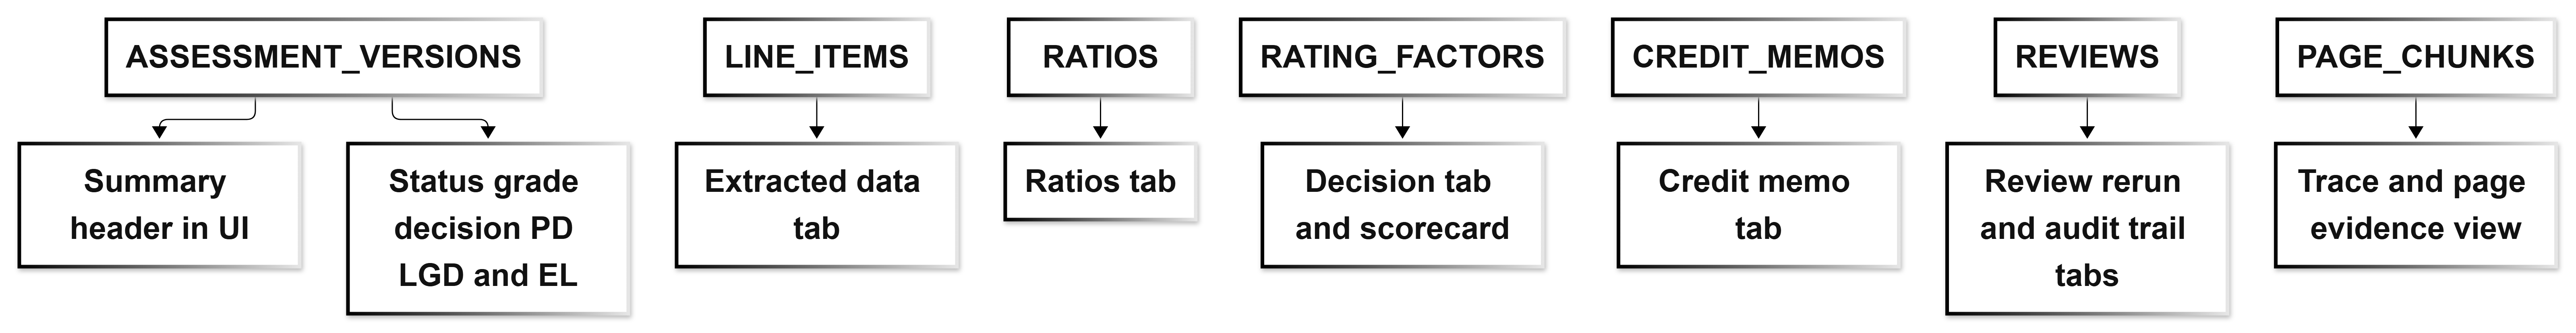
\includegraphics[width=\textwidth,height=0.85\textheight,keepaspectratio]{../diagrams/credit_risk/11_flowchart_10-4-data-flow-from-tables-to-ui.png}
\caption{Data Flow from Tables to UI}
\label{fig:ch04_credit_risk-11-flowchart-10-4-data-flow-from-tables-to-ui}
\end{figure}

\subsection{Modeling Principles}

\speaker{Candidate}{I would follow these principles:}

\begin{enumerate}[leftmargin=\speakwid]
\item One assessment version is the analytical boundary for a single run.
\item Reruns create a new version instead of overwriting the previous version.
\item Every analytical child table joins to the version, not indirectly to another analytical child.
\item Raw JSON is still stored at the version level for completeness, but core objects are normalized for querying.
\item Page-level lineage is preserved for extracted values and score evidence where possible.
\end{enumerate}
\speaker{Interviewer}{Why not store everything only as one big JSON field?}

\speaker{Candidate}{Because the bank will eventually want queries like override rate by grade, average factor contribution by industry, or cases with hard stops and litigation. Pure JSON storage makes those operational analytics harder. A hybrid model works better: normalize core objects, keep the full result JSON for completeness.}
\speaker{Interviewer}{That model is clear. Can you show how the grade, memo, and benchmarks surface in the product screens?}
\speaker{Candidate}{Yes, let's walk through the decision, memo, trend, and benchmark views for the borrower case.}

\medskip\hrule\medskip
\section{Product Screens and Reader Walkthrough}
\label{sec:ch04_credit_risk-11-product-screens-and-reader-walkthrough}

After understanding the data model, it helps readers to see what the final product looks like and how the stored data surfaces in the UI.

\subsection{Main Decision and Scorecard View}

The landing assessment view shows the rating grade, risk band, score, decision, expected loss, and scorecard factors in one place. This helps readers connect the \texttt{assessment\_versions} summary fields and \texttt{rating\_factors} rows to the actual product experience.


\begin{figure}[htbp]
\centering
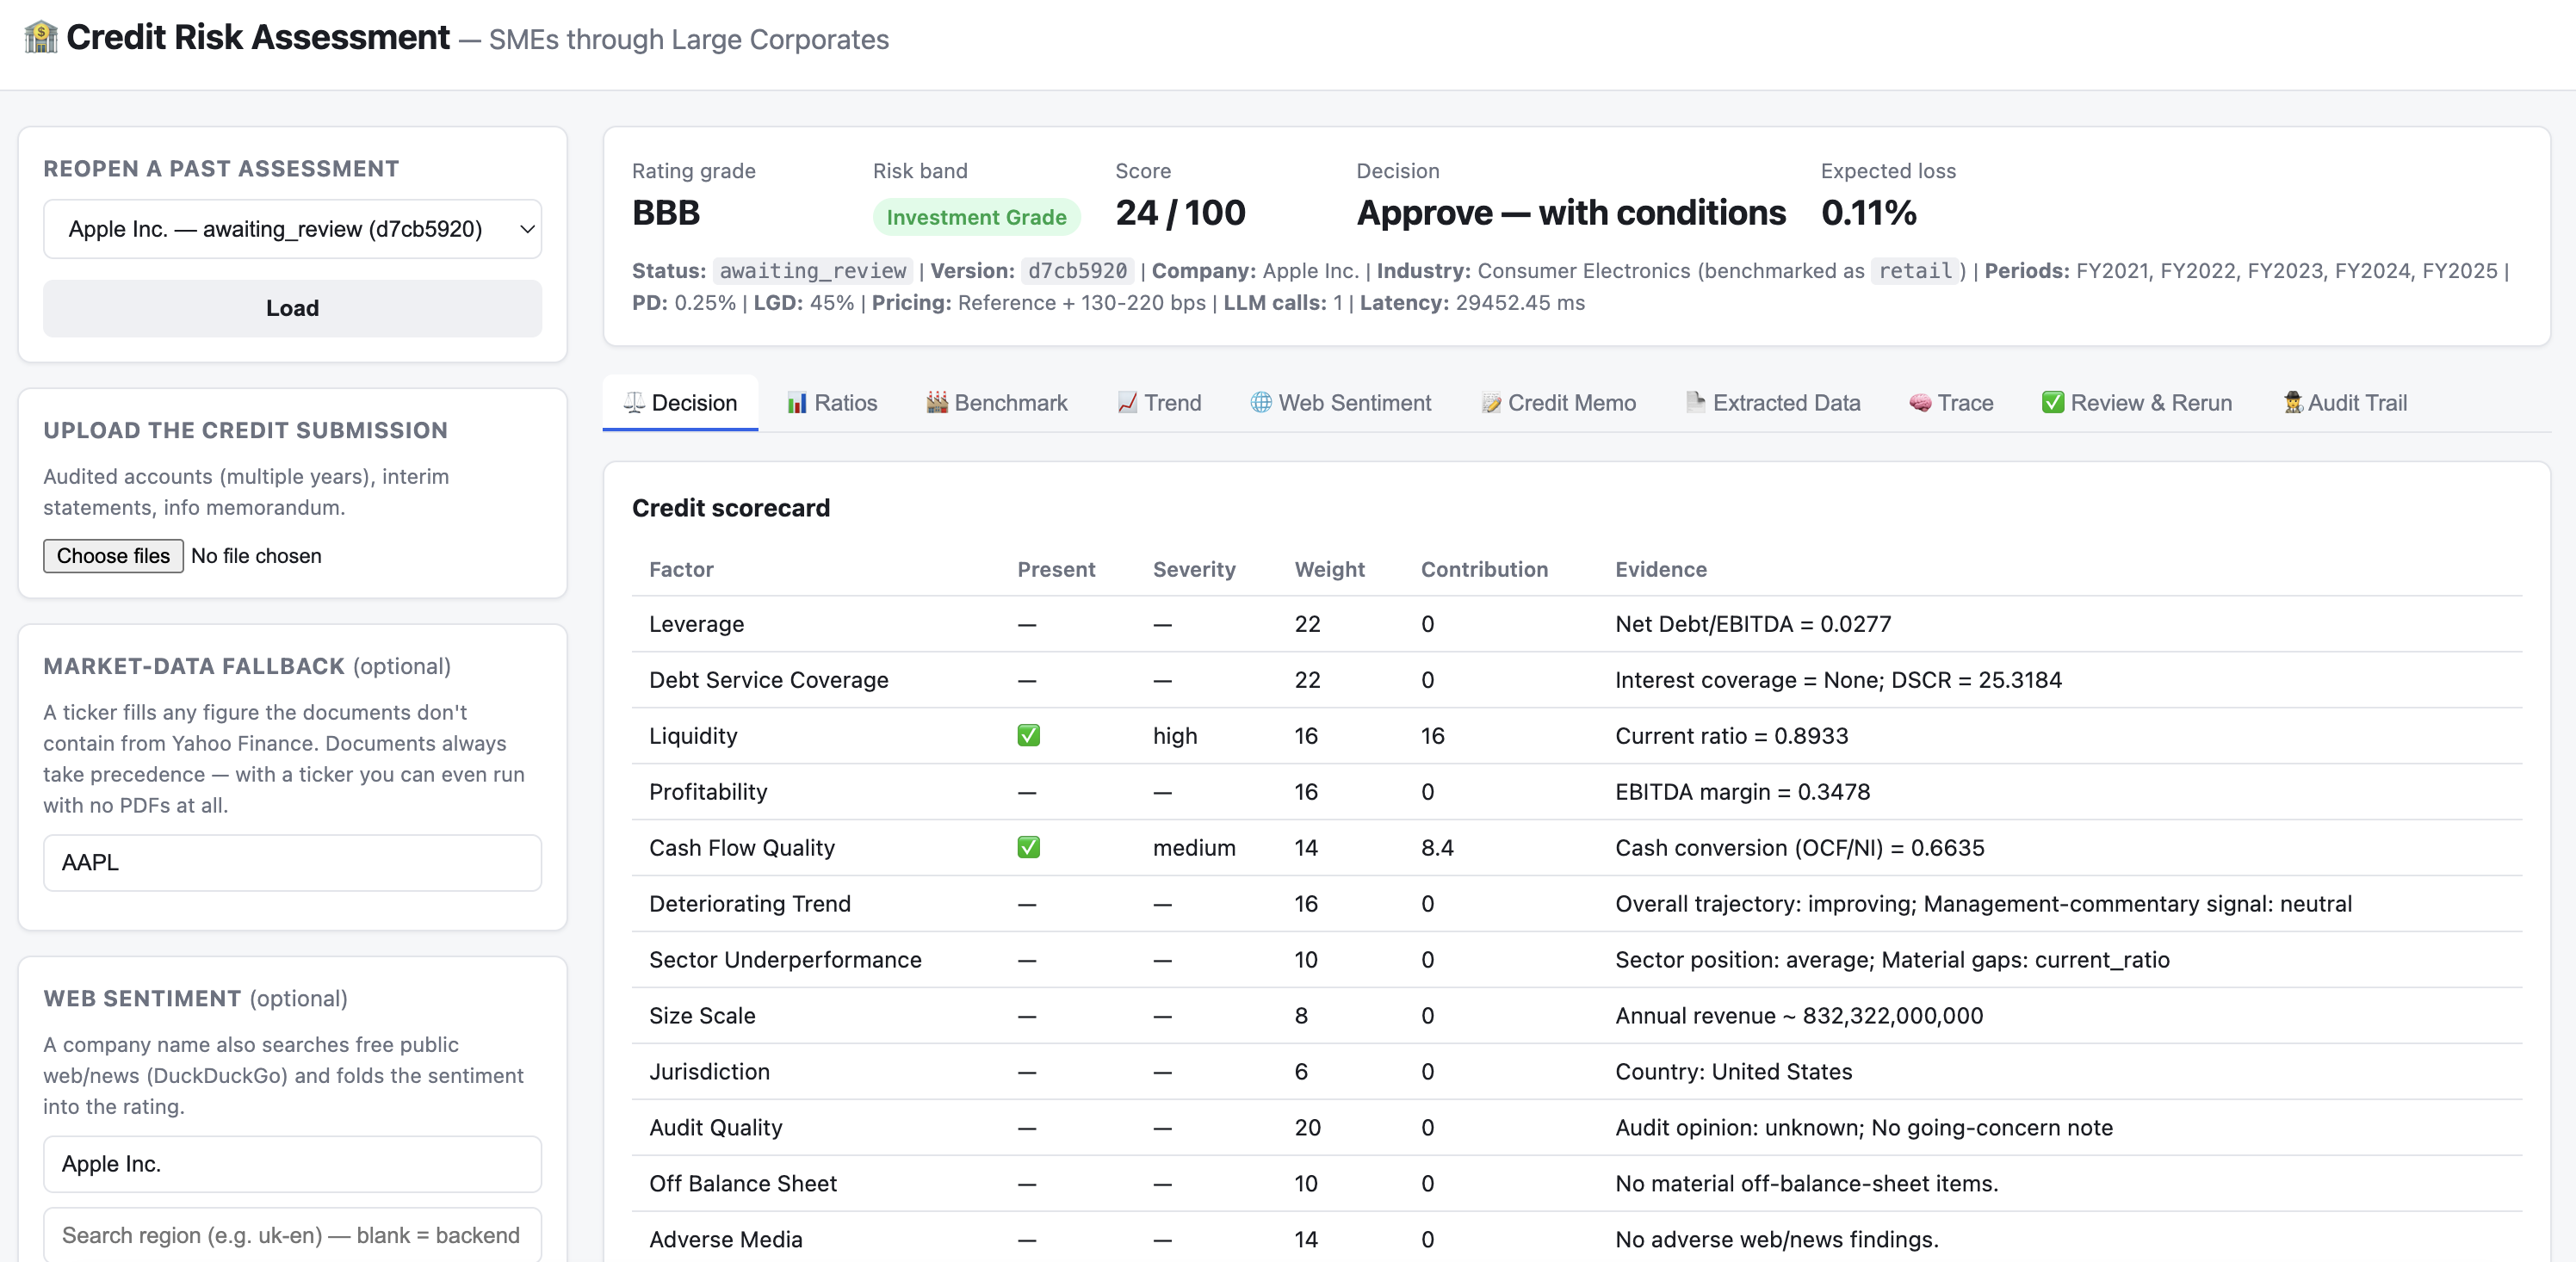
\includegraphics[width=\textwidth,height=0.85\textheight,keepaspectratio]{../diagrams/credit_risk/screen_11_1_decision_scorecard.png}
\caption{Main decision and scorecard view: rating grade, risk band, score, decision, expected loss, and scorecard factors.}
\label{fig:ch04_credit_risk-screen-11-1-decision-scorecard}
\end{figure}

\subsection{Credit Memo View}

The credit memo tab shows the grounded narrative generated from the compact deterministic assessment. This screen is the UI representation of the \texttt{credit\_memos} table and illustrates how the memo stays tied to the computed financial logic instead of raw PDF text.


\begin{figure}[htbp]
\centering
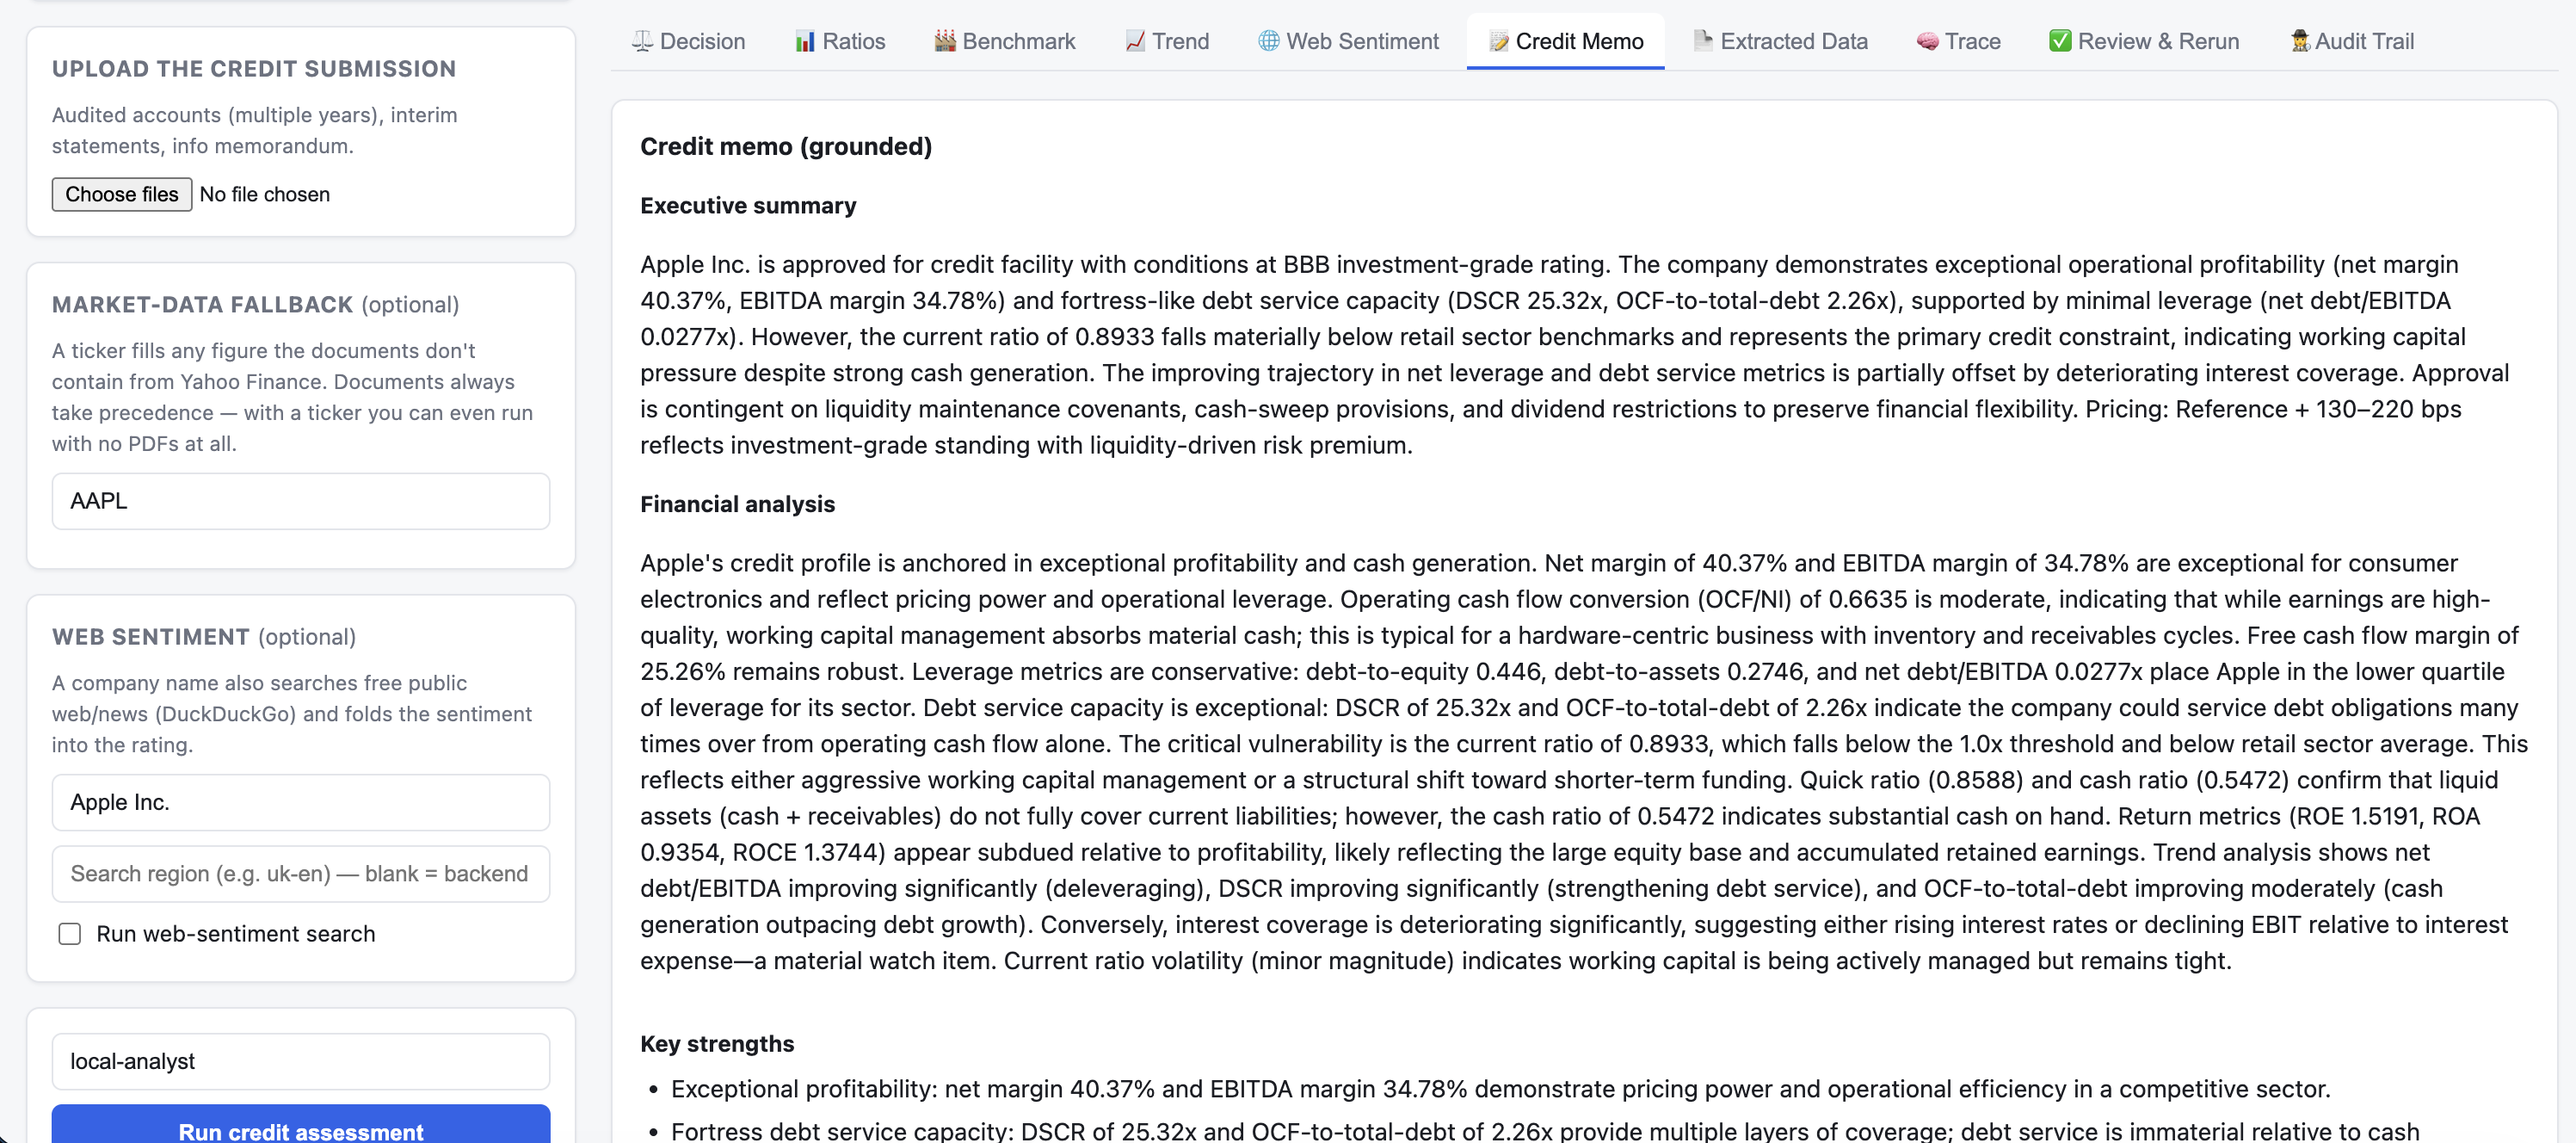
\includegraphics[width=\textwidth,height=0.85\textheight,keepaspectratio]{../diagrams/credit_risk/screen_11_2_credit_memo.png}
\caption{Credit memo view: grounded narrative generated from the compact deterministic assessment.}
\label{fig:ch04_credit_risk-screen-11-2-credit-memo}
\end{figure}

\subsection{Trend Analysis View}

The trend tab shows multi-period ratio movement, direction, magnitude, and percentage change. This helps readers see how the \texttt{ratios} table feeds a user-friendly analytical layer rather than remaining only a backend storage artifact.


\begin{figure}[htbp]
\centering
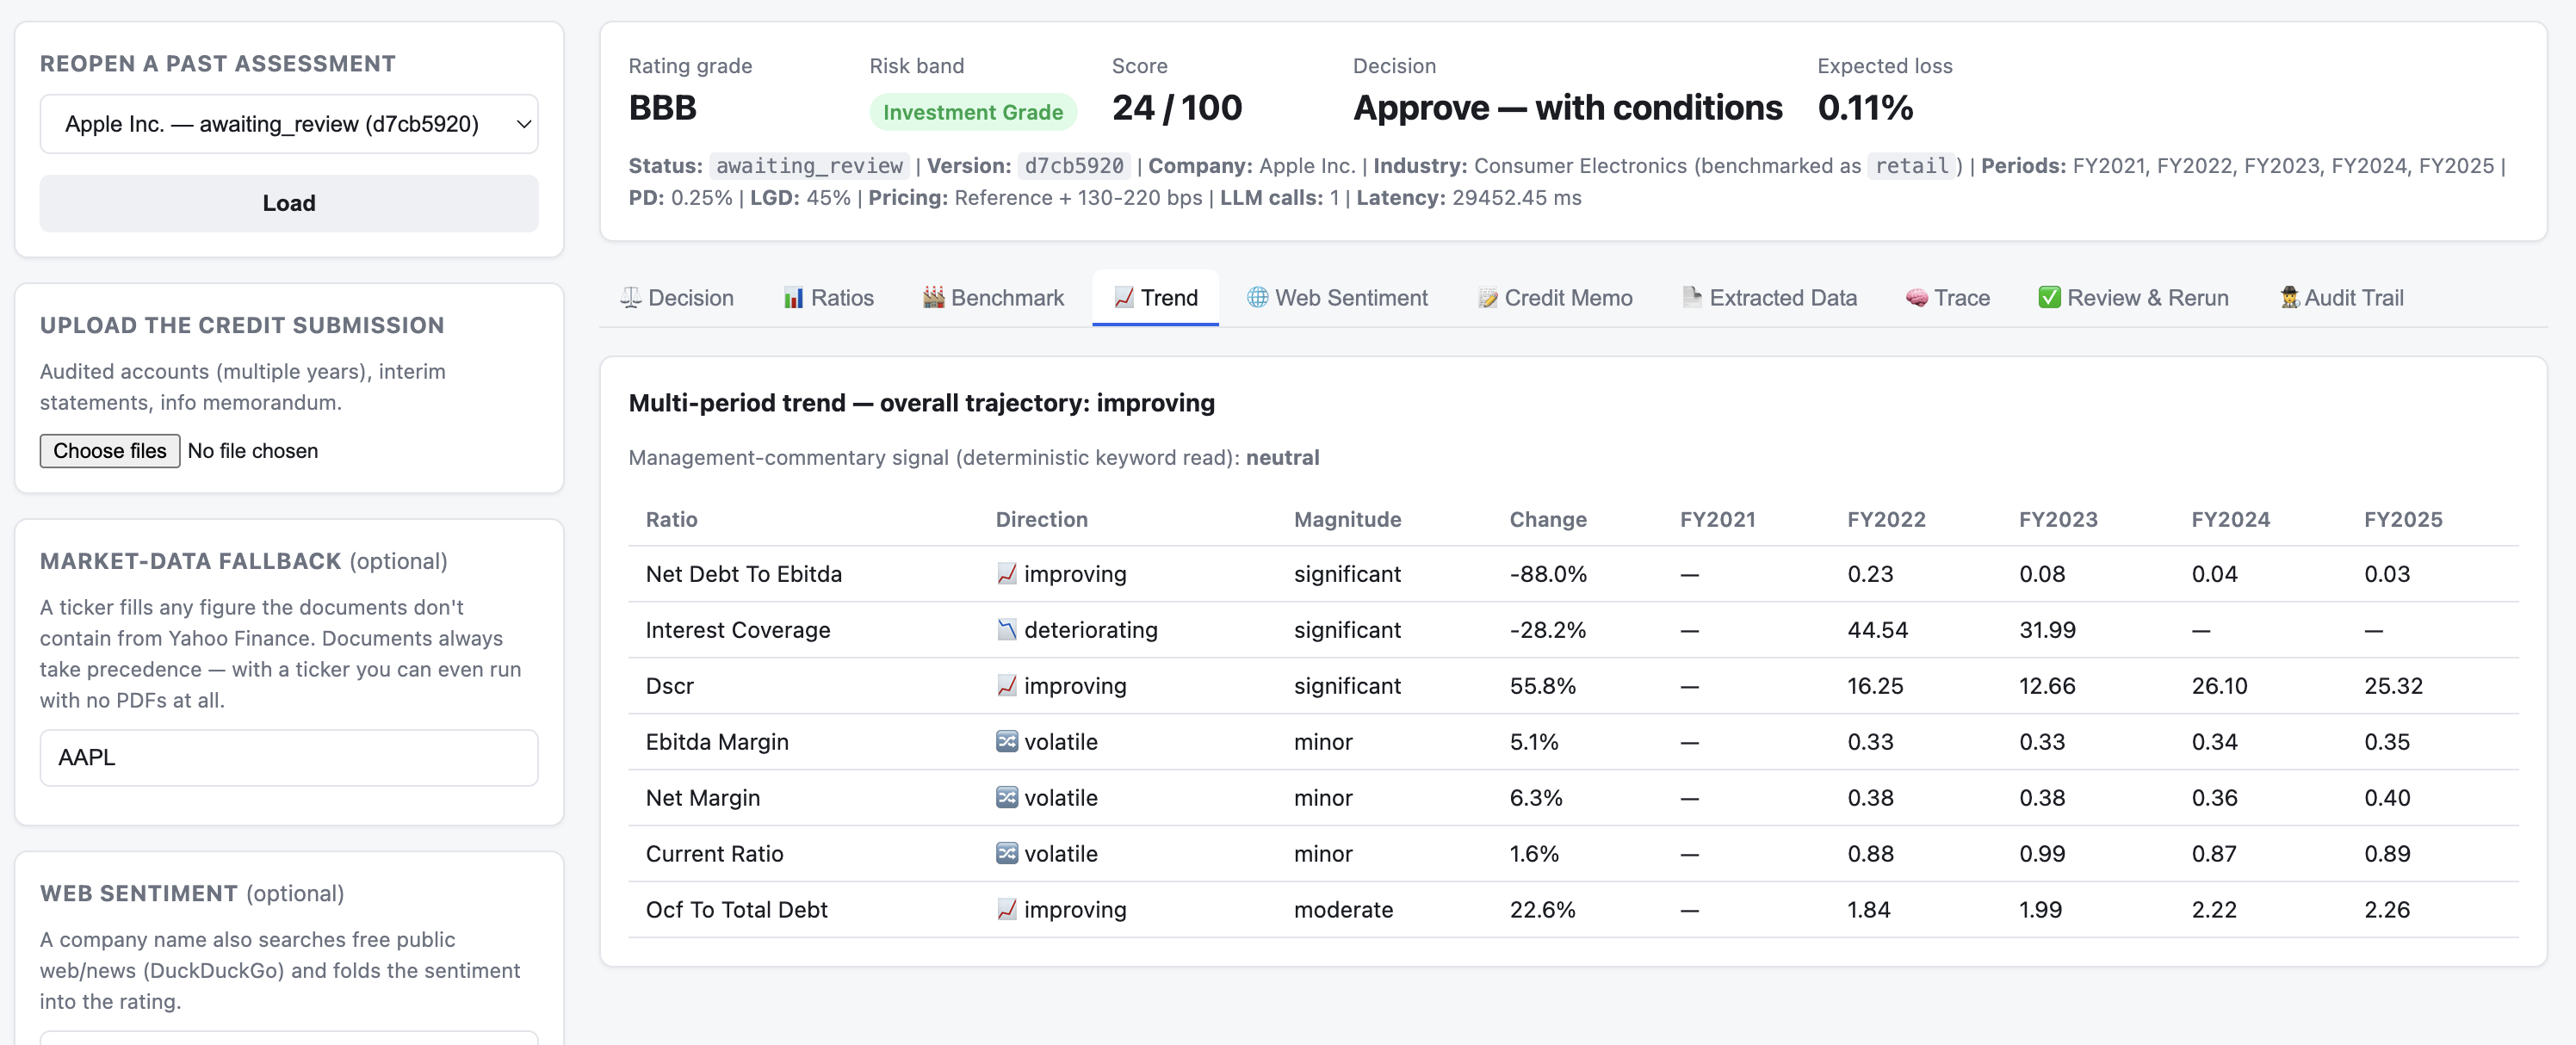
\includegraphics[width=\textwidth,height=0.85\textheight,keepaspectratio]{../diagrams/credit_risk/screen_11_3_trend.png}
\caption{Trend analysis view: multi-period ratio movement with direction, magnitude, and percentage change.}
\label{fig:ch04_credit_risk-screen-11-3-trend}
\end{figure}

\subsection{Sector Benchmark View}

The benchmark screen compares company ratios with sector p25, median, and p75 values, and highlights material gaps. This is a good visual example of how deterministic benchmarking becomes business-readable for analysts and reviewers.


\begin{figure}[htbp]
\centering
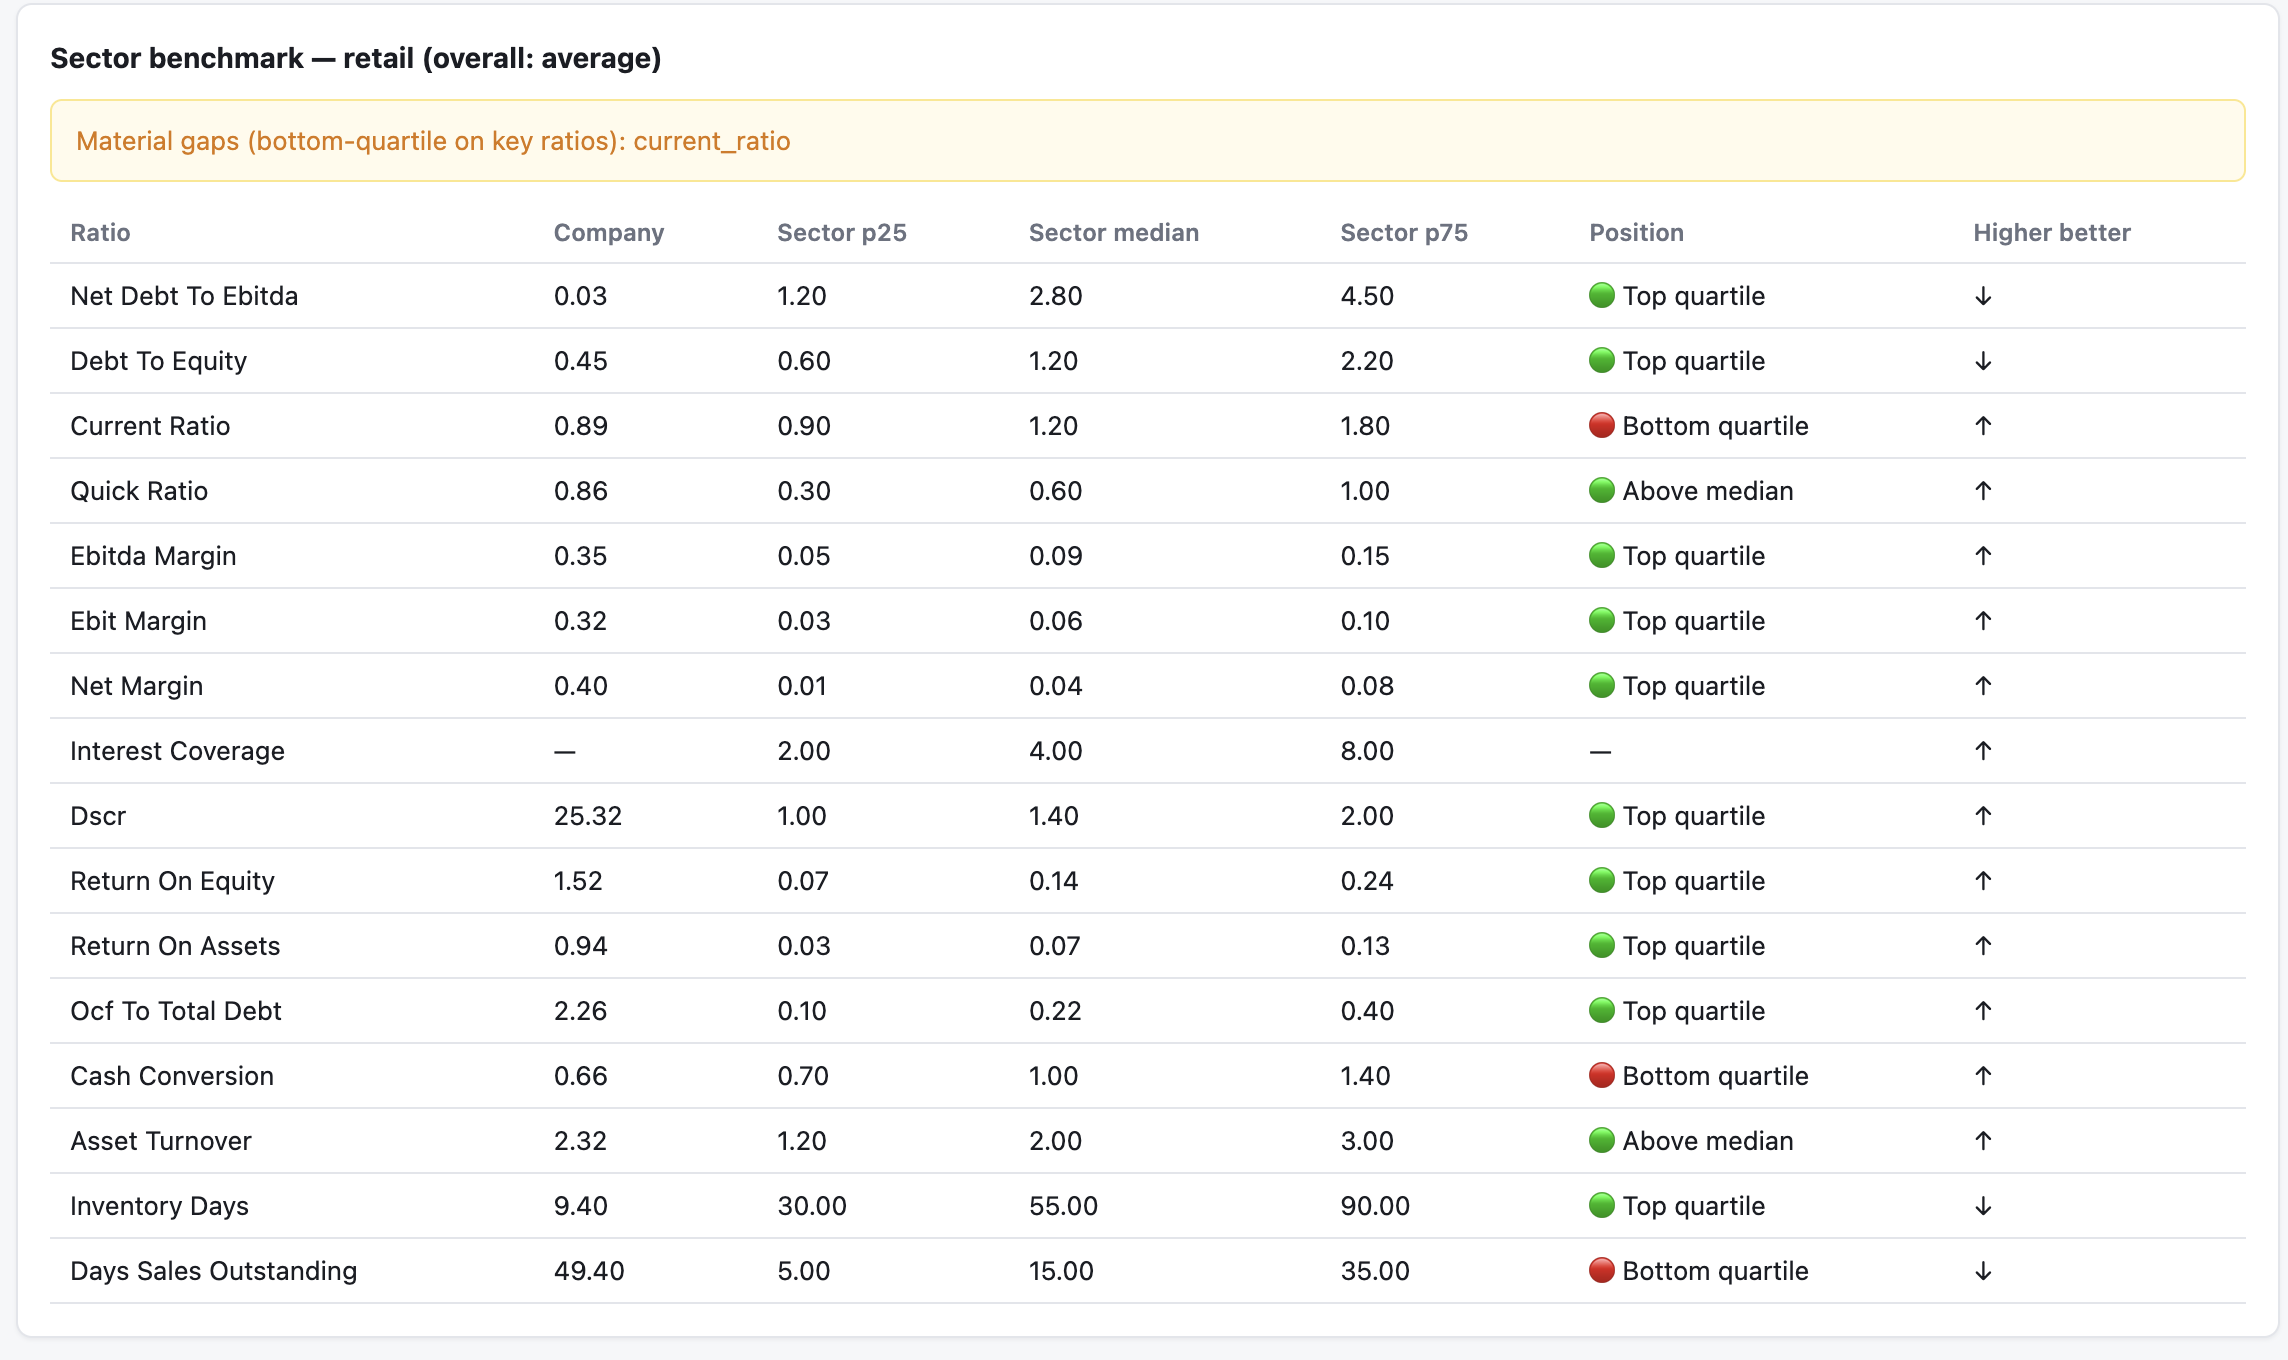
\includegraphics[width=\textwidth,height=0.85\textheight,keepaspectratio]{../diagrams/credit_risk/screen_11_4_benchmark.png}
\caption{Sector benchmark view: company ratios against sector p25, median, and p75 values with material gaps highlighted.}
\label{fig:ch04_credit_risk-screen-11-4-benchmark}
\end{figure}
\speaker{Candidate}{With the borrower views clear, shall we define how to evaluate extraction, scoring, and memo quality next?}

\medskip\hrule\medskip
\section{Evaluation Framework}
\label{sec:ch04_credit_risk-12-evaluation-framework}

\speaker{Interviewer}{Now explain how you would evaluate the system. I do not want only accuracy. I want practical evaluation.}

\speaker{Candidate}{I would evaluate it layer by layer.}

\subsection{Extraction Evaluation}

\begin{itemize}[leftmargin=\speakwid]
\item Company metadata accuracy.
\item Financial line-item extraction accuracy.
\item Notes and contingencies extraction quality.
\item Facility request extraction quality.
\item Period identification correctness.
\item Page lineage correctness.
\end{itemize}
\subsection{Deterministic Validation}

\begin{itemize}[leftmargin=\speakwid]
\item Ratio correctness against manually verified fixtures.
\item Unit normalization correctness.
\item Benchmark classification correctness.
\item Trend classification correctness.
\item Scorecard reproducibility for the same input pack.
\end{itemize}
\subsection{Narrative Evaluation}

\begin{itemize}[leftmargin=\speakwid]
\item Memo completeness.
\item Memo factual consistency with computed scorecard.
\item Unsupported-claim rate.
\item Consistency between active factors and stated risks.
\item Quality of covenant and monitoring trigger recommendations.
\end{itemize}
\subsection{Workflow Evaluation}

\begin{itemize}[leftmargin=\speakwid]
\item Percentage of successful runs.
\item Time from submission to awaiting review.
\item Rate of cases sent to validation review.
\item Rerun success rate.
\item Human approval, rejection, and correction rates.
\end{itemize}
\subsection{Business Evaluation}

\begin{itemize}[leftmargin=\speakwid]
\item Reduction in analyst effort.
\item Turnaround-time reduction.
\item Increase in consistency across memos.
\item Reviewer satisfaction and trust.
\item Audit trace usefulness.
\end{itemize}
\speaker{Interviewer}{How would you create a test dataset?}

\speaker{Candidate}{I would build a golden set of representative credit packs covering different industries, document quality, leverage profiles, audit outcomes, and edge cases. For each case, I would prepare expected extracted values, expected ratios, expected factor severities, and a reviewed reference memo outline.}
\speaker{Candidate}{With evaluation covered, shall we stress-test the design against borrower edge cases and failures next?}

\medskip\hrule\medskip
\section{Edge Cases and Failure Scenarios}
\label{sec:ch04_credit_risk-13-edge-cases-and-failure-scenarios}

\speaker{Interviewer}{Good. Now I want to stress test your design. Let's go through edge cases.}

\subsection{Case 1: No Text in PDF}

\speaker{Interviewer}{What if the analyst uploads a scanned PDF with no text layer?}

\speaker{Candidate}{In my design, the page extraction step should fail clearly and the case should move to validation review or fail-fast, depending on the exact error handling policy. I would not allow downstream extraction to continue on empty content.}

\subsection{Case 2: Missing Facility Letter}

\speaker{Interviewer}{What if the facility request letter is missing?}

\speaker{Candidate}{Then the facility extractor should return nulls for amount, purpose, tenor, and facility type. The system should still complete the run if the rest of the assessment can be built, but the memo should mention missing facility details.}

\subsection{Case 3: Strong Ratios but Going-Concern Note}

\speaker{Interviewer}{Suppose the company looks profitable, but the notes mention going-concern uncertainty. What happens?}

\speaker{Candidate}{The hard-stop logic should dominate. The scorecard should reflect the going-concern disclosure as a critical risk factor and the decision should move to decline or equivalent hard-stop treatment, regardless of favorable ratios.}

\subsection{Case 4: yfinance Disagreement}

\speaker{Interviewer}{What if the extracted revenue from the PDF is 12.4 million but yfinance shows 12.9 million?}

\speaker{Candidate}{If the delta exceeds the discrepancy tolerance, the system should log a discrepancy in reconciliation reasoning. It should not overwrite the document value.}

\subsection{Case 5: Same Company Name in Web Search}

\speaker{Interviewer}{What if a public news result belongs to a different company with a similar name?}

\speaker{Candidate}{That is why the sentiment summarizer must explicitly report disambiguation confidence. Low-confidence evidence should be treated conservatively and never be allowed to strongly drive adverse-media severity.}

\subsection{Case 6: Partial Internal Failure}

\speaker{Interviewer}{What if line items were extracted successfully but the memo step fails?}

\speaker{Candidate}{I would not mark the case as fully complete. The system should either route it to validation review or expose the structured analytical outputs without a final memo, depending on the desired UX. But it must not pretend the full pipeline succeeded.}

\subsection{Case 7: Double Submission}

\speaker{Interviewer}{What if the user double-clicks submit?}

\speaker{Candidate}{Without idempotency, that may create two versions. I would add idempotency keys or duplicate-submission detection for a stronger production design.}

\subsection{Case 8: Low-Confidence Extraction Triggers Retry}

\speaker{Interviewer}{One more: what if the extractor returns JSON that parses but looks untrustworthy, say every label is unknown or the output is empty?}

\speaker{Candidate}{That is exactly what the correctness gate is for. An empty extraction scores 0.0, and unknown labels drag the percent-correct down, so a weak first attempt falls below the 0.50 threshold and the system rebuilds the prompt with the failed validations listed and tries again, bounded at three attempts. For the business this prevents a silent chain reaction where a bad label set produces null ratios, a near-zero score, and a memo that asserts numbers with no grounding. On failure the run keeps the best attempt fail-soft and routes through validation review rather than publishing a confident-looking scorecard, and the four offline gate tests lock this behaviour without needing network access.}
\speaker{Candidate}{With edge cases covered, can we discuss deployment and operations for the assessment service next?}

\medskip\hrule\medskip
\section{Deployment and Operations}
\label{sec:ch04_credit_risk-14-deployment-and-operations}

\speaker{Interviewer}{How would you deploy this?}

\speaker{Candidate}{I would keep deployment simple at first.}

\subsection{Current Operational Shape}

\begin{itemize}[leftmargin=\speakwid]
\item One FastAPI service.
\item Background tasks within the same process.
\item Postgres with pgvector.
\item Redis for status.
\item S3 or ADLS object storage for uploaded documents.
\item Thin web or Streamlit UI.
\end{itemize}
\subsection{Why Single Replica Matters}

\speaker{Candidate}{The workflow is sequential and version-centric, so I would deliberately keep a single service at first for clarity and reproducibility. Document URIs in S3 or ADLS let any replica or worker locate the same files.}

\speaker{Interviewer}{And if we want scale?}

\speaker{Candidate}{Add durable queue workers and scale the application horizontally behind shared object storage and Postgres. That is the cleanest path.}

\subsection{Monitoring Needs}

\begin{itemize}[leftmargin=\speakwid]
\item API health and request metrics.
\item Background job completion and failure counts.
\item LLM call count and latency per assessment.
\item Extraction failure reasons.
\item Redis phase update failures.
\item Review turnaround time.
\item Rerun frequency.
\end{itemize}
\speaker{Candidate}{With deployment and monitoring clear, shall we review the current gaps and enhancement roadmap for the borrower workflow?}

\medskip\hrule\medskip
\section{Current Gaps and Enhancement Roadmap}
\label{sec:ch04_credit_risk-15-current-gaps-and-enhancement-roadmap}

\speaker{Interviewer}{No real system is perfect. What gaps do you see in this design?}

\speaker{Candidate}{Several practical ones.}

\subsection{Current Gaps}

\begin{enumerate}[leftmargin=\speakwid]
\item No OCR for scanned PDFs.
\item No authentication or RBAC hardening.
\item Object storage versioning and lifecycle need hardening for horizontal scaling.
\item No strong idempotency on create.
\item Review approval is not a full workflow engine yet.
\item No advanced retry and backoff around LLM failures.
\item Cost tracking is limited.
\item Validation gates can be stronger.
\end{enumerate}
\subsection{Short-Term Enhancements}

\begin{itemize}[leftmargin=\speakwid]
\item Add OCR support.
\item Add schema-based validation gates after extraction.
\item Add better duplicate-submission protection.
\item Add stronger memo grounding checks.
\end{itemize}
\subsection{Production Enhancements}

\begin{itemize}[leftmargin=\speakwid]
\item Move files to S3 or shared object storage.
\item Add SSO, RBAC, and secret management.
\item Add workflow engine or queue for larger scale.
\item Add formal model and prompt version tracking.
\item Add alerting and dashboards.
\end{itemize}
\subsection{Advanced Enhancements}

\begin{itemize}[leftmargin=\speakwid]
\item Similar borrower retrieval.
\item Portfolio-level concentration analytics.
\item Better policy retrieval and covenant templates.
\item Stronger calibration using historical internal outcomes.
\end{itemize}
\speaker{Candidate}{With the roadmap set, I'm happy to wrap up with final questions on the borrower assessment design.}

\medskip\hrule\medskip
\section{Final Interview Discussion}
\label{sec:ch04_credit_risk-16-final-interview-discussion}

\speaker{Interviewer}{Nice. Let me ask a few final questions quickly.}

\speaker{Interviewer}{Why is this an agentic AI system and not just a normal extraction pipeline?}

\speaker{Candidate}{Because some steps require iterative evidence-seeking behavior. The extraction agents do not just parse a fixed input; they search relevant pages, inspect specific pages, and then return structured outputs. That tool-using, goal-driven behavior is where the agentic pattern adds value.}

\speaker{Interviewer}{Where would you explicitly avoid using the LLM?}

\speaker{Candidate}{Ratio calculation, score mapping, PD/LGD/EL computation, threshold evaluation, and hard-stop logic. Those should remain deterministic.}

\speaker{Interviewer}{Why is human review still mandatory even if the scorecard is deterministic?}

\speaker{Candidate}{Because credit approval is not just mathematics. It includes business judgment, document quality assessment, exceptional situations, and accountability. The system should support the analyst, not replace authorized approvers.}

\speaker{Interviewer}{If I gave you one sentence to summarize the system design, what would it be?}

\speaker{Candidate}{It is a versioned credit assessment platform where agents extract evidence from uploaded financial documents, deterministic Python computes the actual risk analytics, an LLM drafts the memo from those computed results, and a human reviewer remains in control of the final outcome.}

\speaker{Interviewer}{Good. That covers the use case well.}

\speaker{Candidate}{Thank you.}

\section*{Source Code}

The complete implementation for the Credit Risk Assessment Agent is available in the accompanying GitHub repository:

\begin{center}
\url{https://github.com/GSaiDheeraj/Finance-and-Banking-AI-Usecases/tree/main/Credit_Risk_Assesment_Agent}
\end{center}
